% Created by tikzDevice version 0.7.0 on 2014-06-30 20:14:19
% !TEX encoding = UTF-8 Unicode
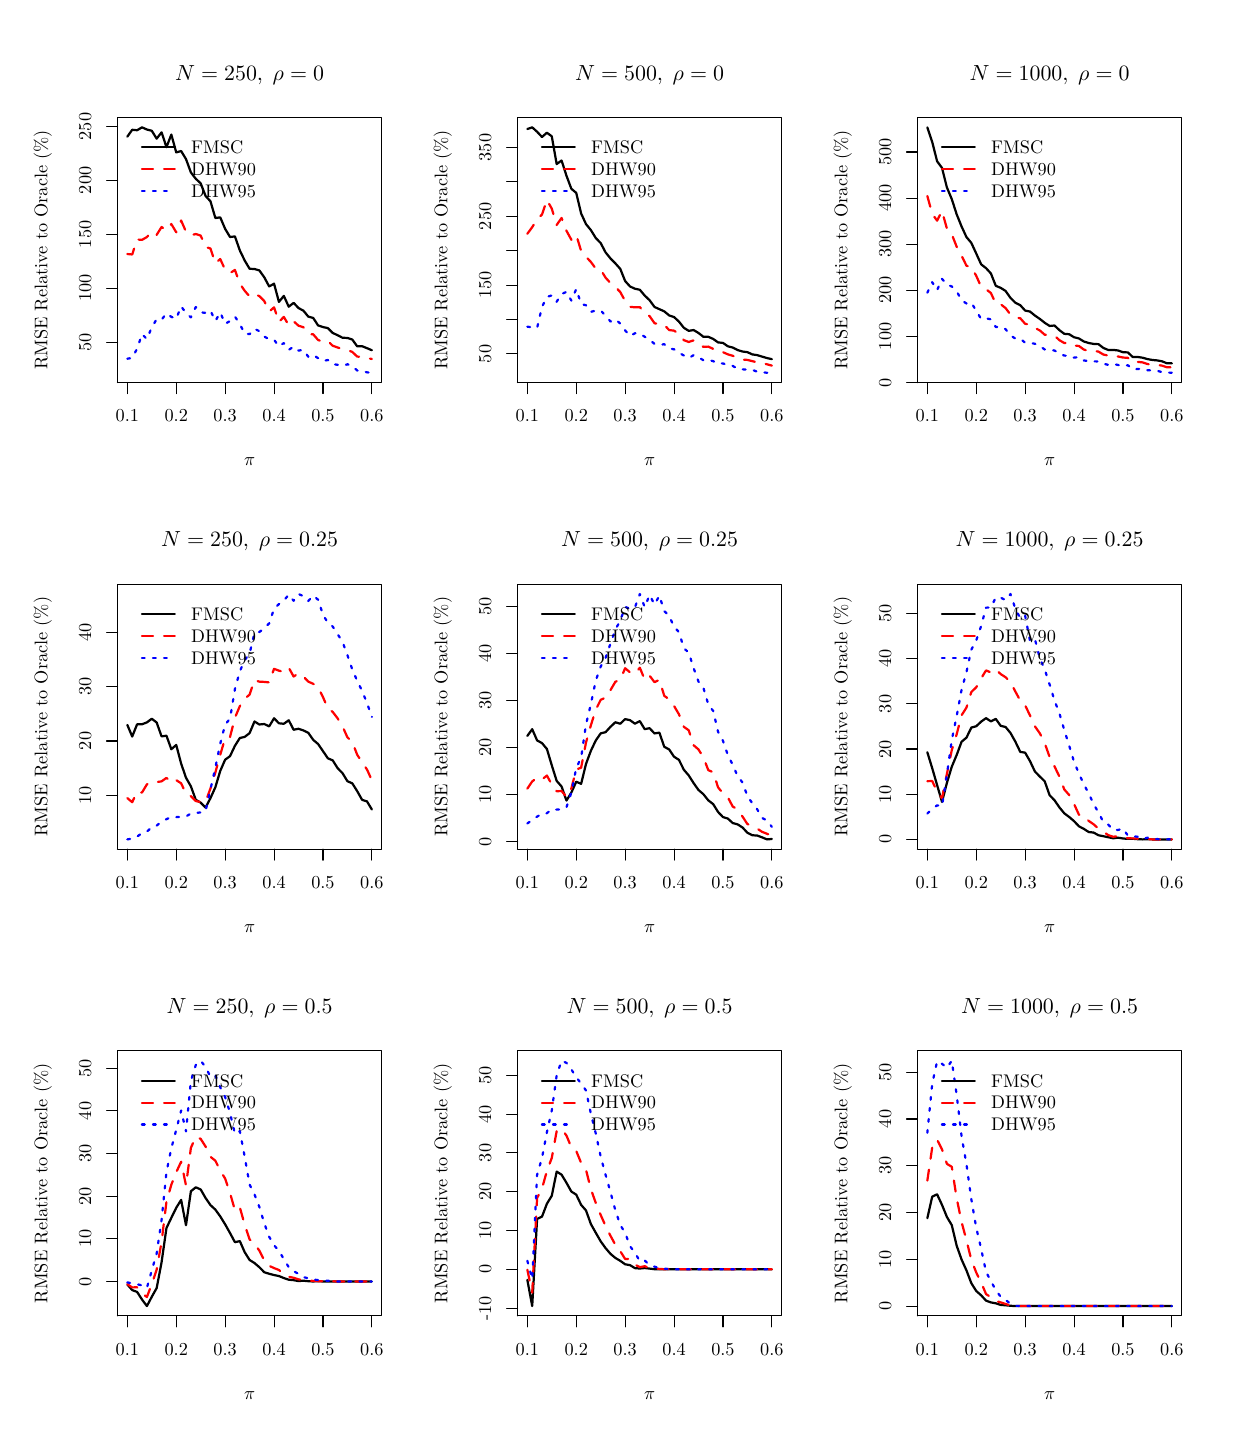
\begin{tikzpicture}[x=1pt,y=1pt]
\definecolor[named]{fillColor}{rgb}{1.00,1.00,1.00}
\path[use as bounding box,fill=fillColor,fill opacity=0.00] (0,0) rectangle (433.62,505.89);
\begin{scope}
\path[clip] ( 32.47,377.65) rectangle (127.91,473.42);
\definecolor[named]{drawColor}{rgb}{0.00,0.00,0.00}

\path[draw=drawColor,line width= 0.8pt,line join=round,line cap=round] ( 36.01,466.50) --
	( 37.77,468.99) --
	( 39.54,468.82) --
	( 41.31,469.87) --
	( 43.08,469.08) --
	( 44.84,468.64) --
	( 46.61,465.78) --
	( 48.38,468.06) --
	( 50.15,462.70) --
	( 51.91,467.27) --
	( 53.68,460.80) --
	( 55.45,461.32) --
	( 57.21,458.40) --
	( 58.98,453.57) --
	( 60.75,451.28) --
	( 62.52,449.63) --
	( 64.28,445.08) --
	( 66.05,443.15) --
	( 67.82,437.11) --
	( 69.59,437.33) --
	( 71.35,433.20) --
	( 73.12,430.23) --
	( 74.89,430.46) --
	( 76.66,425.40) --
	( 78.42,421.75) --
	( 80.19,418.76) --
	( 81.96,418.68) --
	( 83.72,418.17) --
	( 85.49,415.69) --
	( 87.26,412.38) --
	( 89.03,413.37) --
	( 90.79,406.80) --
	( 92.56,408.97) --
	( 94.33,405.06) --
	( 96.10,406.45) --
	( 97.86,404.57) --
	( 99.63,403.63) --
	(101.40,401.48) --
	(103.17,401.00) --
	(104.93,398.30) --
	(106.70,397.70) --
	(108.47,397.32) --
	(110.23,395.57) --
	(112.00,394.75) --
	(113.77,393.83) --
	(115.54,393.77) --
	(117.30,393.19) --
	(119.07,390.74) --
	(120.84,390.78) --
	(122.61,390.08) --
	(124.37,389.32);
\end{scope}
\begin{scope}
\path[clip] (  0.00,  0.00) rectangle (433.62,505.89);
\definecolor[named]{drawColor}{rgb}{0.00,0.00,0.00}

\path[draw=drawColor,line width= 0.4pt,line join=round,line cap=round] ( 36.01,377.65) -- (124.37,377.65);

\path[draw=drawColor,line width= 0.4pt,line join=round,line cap=round] ( 36.01,377.65) -- ( 36.01,373.69);

\path[draw=drawColor,line width= 0.4pt,line join=round,line cap=round] ( 53.68,377.65) -- ( 53.68,373.69);

\path[draw=drawColor,line width= 0.4pt,line join=round,line cap=round] ( 71.35,377.65) -- ( 71.35,373.69);

\path[draw=drawColor,line width= 0.4pt,line join=round,line cap=round] ( 89.03,377.65) -- ( 89.03,373.69);

\path[draw=drawColor,line width= 0.4pt,line join=round,line cap=round] (106.70,377.65) -- (106.70,373.69);

\path[draw=drawColor,line width= 0.4pt,line join=round,line cap=round] (124.37,377.65) -- (124.37,373.69);

\node[text=drawColor,anchor=base,inner sep=0pt, outer sep=0pt, scale=  0.66] at ( 36.01,363.40) {0.1};

\node[text=drawColor,anchor=base,inner sep=0pt, outer sep=0pt, scale=  0.66] at ( 53.68,363.40) {0.2};

\node[text=drawColor,anchor=base,inner sep=0pt, outer sep=0pt, scale=  0.66] at ( 71.35,363.40) {0.3};

\node[text=drawColor,anchor=base,inner sep=0pt, outer sep=0pt, scale=  0.66] at ( 89.03,363.40) {0.4};

\node[text=drawColor,anchor=base,inner sep=0pt, outer sep=0pt, scale=  0.66] at (106.70,363.40) {0.5};

\node[text=drawColor,anchor=base,inner sep=0pt, outer sep=0pt, scale=  0.66] at (124.37,363.40) {0.6};

\path[draw=drawColor,line width= 0.4pt,line join=round,line cap=round] ( 32.47,392.27) -- ( 32.47,470.18);

\path[draw=drawColor,line width= 0.4pt,line join=round,line cap=round] ( 32.47,392.27) -- ( 28.51,392.27);

\path[draw=drawColor,line width= 0.4pt,line join=round,line cap=round] ( 32.47,411.75) -- ( 28.51,411.75);

\path[draw=drawColor,line width= 0.4pt,line join=round,line cap=round] ( 32.47,431.22) -- ( 28.51,431.22);

\path[draw=drawColor,line width= 0.4pt,line join=round,line cap=round] ( 32.47,450.70) -- ( 28.51,450.70);

\path[draw=drawColor,line width= 0.4pt,line join=round,line cap=round] ( 32.47,470.18) -- ( 28.51,470.18);

\node[text=drawColor,rotate= 90.00,anchor=base,inner sep=0pt, outer sep=0pt, scale=  0.66] at ( 22.97,392.27) {50};

\node[text=drawColor,rotate= 90.00,anchor=base,inner sep=0pt, outer sep=0pt, scale=  0.66] at ( 22.97,411.75) {100};

\node[text=drawColor,rotate= 90.00,anchor=base,inner sep=0pt, outer sep=0pt, scale=  0.66] at ( 22.97,431.22) {150};

\node[text=drawColor,rotate= 90.00,anchor=base,inner sep=0pt, outer sep=0pt, scale=  0.66] at ( 22.97,450.70) {200};

\node[text=drawColor,rotate= 90.00,anchor=base,inner sep=0pt, outer sep=0pt, scale=  0.66] at ( 22.97,470.18) {250};

\path[draw=drawColor,line width= 0.4pt,line join=round,line cap=round] ( 32.47,377.65) --
	(127.91,377.65) --
	(127.91,473.42) --
	( 32.47,473.42) --
	( 32.47,377.65);
\end{scope}
\begin{scope}
\path[clip] (  0.00,337.26) rectangle (144.54,505.89);
\definecolor[named]{drawColor}{rgb}{0.00,0.00,0.00}

\node[text=drawColor,anchor=base,inner sep=0pt, outer sep=0pt, scale=  0.79] at ( 80.19,486.92) {\bfseries $N=250, \;\rho=0$};

\node[text=drawColor,anchor=base,inner sep=0pt, outer sep=0pt, scale=  0.66] at ( 80.19,347.56) {$\pi$};

\node[text=drawColor,rotate= 90.00,anchor=base,inner sep=0pt, outer sep=0pt, scale=  0.66] at (  7.13,425.53) {RMSE Relative to Oracle (\%)};
\end{scope}
\begin{scope}
\path[clip] ( 32.47,377.65) rectangle (127.91,473.42);
\definecolor[named]{drawColor}{rgb}{1.00,0.00,0.00}

\path[draw=drawColor,line width= 0.8pt,dash pattern=on 4pt off 4pt ,line join=round,line cap=round] ( 36.01,424.09) --
	( 37.77,423.93) --
	( 39.54,429.35) --
	( 41.31,429.20) --
	( 43.08,430.23) --
	( 44.84,432.19) --
	( 46.61,431.03) --
	( 48.38,433.85) --
	( 50.15,432.69) --
	( 51.91,434.93) --
	( 53.68,431.95) --
	( 55.45,436.20) --
	( 57.21,432.17) --
	( 58.98,430.86) --
	( 60.75,431.32) --
	( 62.52,430.75) --
	( 64.28,426.63) --
	( 66.05,426.09) --
	( 67.82,420.75) --
	( 69.59,422.28) --
	( 71.35,418.38) --
	( 73.12,417.19) --
	( 74.89,418.35) --
	( 76.66,413.39) --
	( 78.42,410.81) --
	( 80.19,408.76) --
	( 81.96,409.68) --
	( 83.72,408.87) --
	( 85.49,407.10) --
	( 87.26,403.28) --
	( 89.03,404.82) --
	( 90.79,399.52) --
	( 92.56,401.38) --
	( 94.33,398.33) --
	( 96.10,399.79) --
	( 97.86,398.20) --
	( 99.63,397.63) --
	(101.40,395.14) --
	(103.17,395.09) --
	(104.93,393.03) --
	(106.70,392.37) --
	(108.47,392.61) --
	(110.23,390.94) --
	(112.00,390.32) --
	(113.77,389.76) --
	(115.54,389.41) --
	(117.30,388.71) --
	(119.07,387.04) --
	(120.84,386.90) --
	(122.61,386.52) --
	(124.37,386.17);
\definecolor[named]{drawColor}{rgb}{0.00,0.00,1.00}

\path[draw=drawColor,line width= 0.8pt,dash pattern=on 1pt off 3pt ,line join=round,line cap=round] ( 36.01,386.26) --
	( 37.77,386.55) --
	( 39.54,389.89) --
	( 41.31,395.15) --
	( 43.08,393.36) --
	( 44.84,397.60) --
	( 46.61,400.55) --
	( 48.38,400.34) --
	( 50.15,402.66) --
	( 51.91,401.39) --
	( 53.68,400.69) --
	( 55.45,405.20) --
	( 57.21,402.74) --
	( 58.98,401.21) --
	( 60.75,404.93) --
	( 62.52,403.02) --
	( 64.28,402.82) --
	( 66.05,403.64) --
	( 67.82,399.88) --
	( 69.59,402.98) --
	( 71.35,398.87) --
	( 73.12,399.89) --
	( 74.89,401.49) --
	( 76.66,398.81) --
	( 78.42,395.31) --
	( 80.19,395.15) --
	( 81.96,397.07) --
	( 83.72,396.22) --
	( 85.49,394.29) --
	( 87.26,393.28) --
	( 89.03,393.10) --
	( 90.79,390.73) --
	( 92.56,391.93) --
	( 94.33,389.46) --
	( 96.10,390.62) --
	( 97.86,389.21) --
	( 99.63,389.44) --
	(101.40,386.97) --
	(103.17,387.66) --
	(104.93,386.46) --
	(106.70,385.45) --
	(108.47,385.79) --
	(110.23,384.32) --
	(112.00,384.06) --
	(113.77,383.68) --
	(115.54,384.25) --
	(117.30,383.63) --
	(119.07,382.00) --
	(120.84,381.80) --
	(122.61,381.34) --
	(124.37,381.20);
\definecolor[named]{drawColor}{rgb}{0.00,0.00,0.00}

\path[draw=drawColor,line width= 0.8pt,line join=round,line cap=round] ( 41.28,462.63) -- ( 53.16,462.63);
\definecolor[named]{drawColor}{rgb}{1.00,0.00,0.00}

\path[draw=drawColor,line width= 0.8pt,dash pattern=on 4pt off 4pt ,line join=round,line cap=round] ( 41.28,454.71) -- ( 53.16,454.71);
\definecolor[named]{drawColor}{rgb}{0.00,0.00,1.00}

\path[draw=drawColor,line width= 0.8pt,dash pattern=on 1pt off 3pt ,line join=round,line cap=round] ( 41.28,446.79) -- ( 53.16,446.79);
\definecolor[named]{drawColor}{rgb}{0.00,0.00,0.00}

\node[text=drawColor,anchor=base west,inner sep=0pt, outer sep=0pt, scale=  0.66] at ( 59.10,460.35) {FMSC};

\node[text=drawColor,anchor=base west,inner sep=0pt, outer sep=0pt, scale=  0.66] at ( 59.10,452.43) {DHW90};

\node[text=drawColor,anchor=base west,inner sep=0pt, outer sep=0pt, scale=  0.66] at ( 59.10,444.51) {DHW95};
\end{scope}
\begin{scope}
\path[clip] (177.01,377.65) rectangle (272.45,473.42);
\definecolor[named]{drawColor}{rgb}{0.00,0.00,0.00}

\path[draw=drawColor,line width= 0.8pt,line join=round,line cap=round] (180.55,469.26) --
	(182.31,469.87) --
	(184.08,468.27) --
	(185.85,466.38) --
	(187.62,467.93) --
	(189.38,466.64) --
	(191.15,456.59) --
	(192.92,457.89) --
	(194.69,452.39) --
	(196.45,447.68) --
	(198.22,446.19) --
	(199.99,438.74) --
	(201.75,434.90) --
	(203.52,432.73) --
	(205.29,429.86) --
	(207.06,428.05) --
	(208.82,424.69) --
	(210.59,422.49) --
	(212.36,420.71) --
	(214.13,418.72) --
	(215.89,414.33) --
	(217.66,412.37) --
	(219.43,411.55) --
	(221.20,411.18) --
	(222.96,409.08) --
	(224.73,407.39) --
	(226.50,404.97) --
	(228.26,404.17) --
	(230.03,403.37) --
	(231.80,401.90) --
	(233.57,401.31) --
	(235.33,399.68) --
	(237.10,397.44) --
	(238.87,396.33) --
	(240.64,396.62) --
	(242.40,395.57) --
	(244.17,394.18) --
	(245.94,394.18) --
	(247.71,393.41) --
	(249.47,392.16) --
	(251.24,391.97) --
	(253.01,390.75) --
	(254.77,390.31) --
	(256.54,389.39) --
	(258.31,388.86) --
	(260.08,388.63) --
	(261.84,387.82) --
	(263.61,387.56) --
	(265.38,387.02) --
	(267.15,386.50) --
	(268.91,386.10);
\end{scope}
\begin{scope}
\path[clip] (  0.00,  0.00) rectangle (433.62,505.89);
\definecolor[named]{drawColor}{rgb}{0.00,0.00,0.00}

\path[draw=drawColor,line width= 0.4pt,line join=round,line cap=round] (180.55,377.65) -- (268.91,377.65);

\path[draw=drawColor,line width= 0.4pt,line join=round,line cap=round] (180.55,377.65) -- (180.55,373.69);

\path[draw=drawColor,line width= 0.4pt,line join=round,line cap=round] (198.22,377.65) -- (198.22,373.69);

\path[draw=drawColor,line width= 0.4pt,line join=round,line cap=round] (215.89,377.65) -- (215.89,373.69);

\path[draw=drawColor,line width= 0.4pt,line join=round,line cap=round] (233.57,377.65) -- (233.57,373.69);

\path[draw=drawColor,line width= 0.4pt,line join=round,line cap=round] (251.24,377.65) -- (251.24,373.69);

\path[draw=drawColor,line width= 0.4pt,line join=round,line cap=round] (268.91,377.65) -- (268.91,373.69);

\node[text=drawColor,anchor=base,inner sep=0pt, outer sep=0pt, scale=  0.66] at (180.55,363.40) {0.1};

\node[text=drawColor,anchor=base,inner sep=0pt, outer sep=0pt, scale=  0.66] at (198.22,363.40) {0.2};

\node[text=drawColor,anchor=base,inner sep=0pt, outer sep=0pt, scale=  0.66] at (215.89,363.40) {0.3};

\node[text=drawColor,anchor=base,inner sep=0pt, outer sep=0pt, scale=  0.66] at (233.57,363.40) {0.4};

\node[text=drawColor,anchor=base,inner sep=0pt, outer sep=0pt, scale=  0.66] at (251.24,363.40) {0.5};

\node[text=drawColor,anchor=base,inner sep=0pt, outer sep=0pt, scale=  0.66] at (268.91,363.40) {0.6};

\path[draw=drawColor,line width= 0.4pt,line join=round,line cap=round] (177.01,388.00) -- (177.01,462.59);

\path[draw=drawColor,line width= 0.4pt,line join=round,line cap=round] (177.01,388.00) -- (173.05,388.00);

\path[draw=drawColor,line width= 0.4pt,line join=round,line cap=round] (177.01,400.43) -- (173.05,400.43);

\path[draw=drawColor,line width= 0.4pt,line join=round,line cap=round] (177.01,412.86) -- (173.05,412.86);

\path[draw=drawColor,line width= 0.4pt,line join=round,line cap=round] (177.01,425.29) -- (173.05,425.29);

\path[draw=drawColor,line width= 0.4pt,line join=round,line cap=round] (177.01,437.72) -- (173.05,437.72);

\path[draw=drawColor,line width= 0.4pt,line join=round,line cap=round] (177.01,450.15) -- (173.05,450.15);

\path[draw=drawColor,line width= 0.4pt,line join=round,line cap=round] (177.01,462.59) -- (173.05,462.59);

\node[text=drawColor,rotate= 90.00,anchor=base,inner sep=0pt, outer sep=0pt, scale=  0.66] at (167.51,388.00) {50};

\node[text=drawColor,rotate= 90.00,anchor=base,inner sep=0pt, outer sep=0pt, scale=  0.66] at (167.51,412.86) {150};

\node[text=drawColor,rotate= 90.00,anchor=base,inner sep=0pt, outer sep=0pt, scale=  0.66] at (167.51,437.72) {250};

\node[text=drawColor,rotate= 90.00,anchor=base,inner sep=0pt, outer sep=0pt, scale=  0.66] at (167.51,462.59) {350};

\path[draw=drawColor,line width= 0.4pt,line join=round,line cap=round] (177.01,377.65) --
	(272.45,377.65) --
	(272.45,473.42) --
	(177.01,473.42) --
	(177.01,377.65);
\end{scope}
\begin{scope}
\path[clip] (144.54,337.26) rectangle (289.08,505.89);
\definecolor[named]{drawColor}{rgb}{0.00,0.00,0.00}

\node[text=drawColor,anchor=base,inner sep=0pt, outer sep=0pt, scale=  0.79] at (224.73,486.92) {\bfseries $N=500, \;\rho=0$};

\node[text=drawColor,anchor=base,inner sep=0pt, outer sep=0pt, scale=  0.66] at (224.73,347.56) {$\pi$};

\node[text=drawColor,rotate= 90.00,anchor=base,inner sep=0pt, outer sep=0pt, scale=  0.66] at (151.67,425.53) {RMSE Relative to Oracle (\%)};
\end{scope}
\begin{scope}
\path[clip] (177.01,377.65) rectangle (272.45,473.42);
\definecolor[named]{drawColor}{rgb}{1.00,0.00,0.00}

\path[draw=drawColor,line width= 0.8pt,dash pattern=on 4pt off 4pt ,line join=round,line cap=round] (180.55,431.40) --
	(182.31,433.79) --
	(184.08,436.64) --
	(185.85,438.38) --
	(187.62,443.64) --
	(189.38,440.50) --
	(191.15,434.60) --
	(192.92,437.13) --
	(194.69,432.50) --
	(196.45,429.26) --
	(198.22,431.04) --
	(199.99,425.19) --
	(201.75,423.11) --
	(203.52,421.22) --
	(205.29,418.82) --
	(207.06,418.44) --
	(208.82,415.55) --
	(210.59,413.60) --
	(212.36,412.20) --
	(214.13,410.34) --
	(215.89,407.14) --
	(217.66,405.01) --
	(219.43,404.83) --
	(221.20,404.91) --
	(222.96,402.71) --
	(224.73,401.65) --
	(226.50,399.10) --
	(228.26,398.66) --
	(230.03,398.47) --
	(231.80,396.61) --
	(233.57,396.41) --
	(235.33,395.24) --
	(237.10,392.97) --
	(238.87,392.31) --
	(240.64,392.89) --
	(242.40,391.90) --
	(244.17,390.54) --
	(245.94,390.64) --
	(247.71,389.81) --
	(249.47,388.69) --
	(251.24,388.63) --
	(253.01,387.83) --
	(254.77,387.32) --
	(256.54,386.58) --
	(258.31,385.95) --
	(260.08,385.83) --
	(261.84,385.39) --
	(263.61,384.94) --
	(265.38,384.72) --
	(267.15,384.25) --
	(268.91,383.77);
\definecolor[named]{drawColor}{rgb}{0.00,0.00,1.00}

\path[draw=drawColor,line width= 0.8pt,dash pattern=on 1pt off 3pt ,line join=round,line cap=round] (180.55,397.83) --
	(182.31,397.61) --
	(184.08,397.41) --
	(185.85,405.02) --
	(187.62,408.59) --
	(189.38,409.15) --
	(191.15,406.87) --
	(192.92,409.65) --
	(194.69,410.41) --
	(196.45,407.29) --
	(198.22,411.43) --
	(199.99,406.05) --
	(201.75,405.56) --
	(203.52,403.20) --
	(205.29,403.66) --
	(207.06,403.67) --
	(208.82,401.83) --
	(210.59,399.70) --
	(212.36,400.54) --
	(214.13,398.95) --
	(215.89,396.50) --
	(217.66,394.49) --
	(219.43,395.46) --
	(221.20,395.36) --
	(222.96,394.20) --
	(224.73,393.04) --
	(226.50,391.64) --
	(228.26,391.18) --
	(230.03,391.52) --
	(231.80,390.01) --
	(233.57,389.65) --
	(235.33,388.38) --
	(237.10,387.44) --
	(238.87,386.52) --
	(240.64,387.55) --
	(242.40,386.84) --
	(244.17,385.68) --
	(245.94,385.82) --
	(247.71,385.39) --
	(249.47,384.45) --
	(251.24,384.57) --
	(253.01,383.88) --
	(254.77,383.65) --
	(256.54,382.65) --
	(258.31,382.43) --
	(260.08,382.29) --
	(261.84,382.25) --
	(263.61,381.55) --
	(265.38,381.35) --
	(267.15,381.20) --
	(268.91,381.20);
\definecolor[named]{drawColor}{rgb}{0.00,0.00,0.00}

\path[draw=drawColor,line width= 0.8pt,line join=round,line cap=round] (185.82,462.63) -- (197.70,462.63);
\definecolor[named]{drawColor}{rgb}{1.00,0.00,0.00}

\path[draw=drawColor,line width= 0.8pt,dash pattern=on 4pt off 4pt ,line join=round,line cap=round] (185.82,454.71) -- (197.70,454.71);
\definecolor[named]{drawColor}{rgb}{0.00,0.00,1.00}

\path[draw=drawColor,line width= 0.8pt,dash pattern=on 1pt off 3pt ,line join=round,line cap=round] (185.82,446.79) -- (197.70,446.79);
\definecolor[named]{drawColor}{rgb}{0.00,0.00,0.00}

\node[text=drawColor,anchor=base west,inner sep=0pt, outer sep=0pt, scale=  0.66] at (203.64,460.35) {FMSC};

\node[text=drawColor,anchor=base west,inner sep=0pt, outer sep=0pt, scale=  0.66] at (203.64,452.43) {DHW90};

\node[text=drawColor,anchor=base west,inner sep=0pt, outer sep=0pt, scale=  0.66] at (203.64,444.51) {DHW95};
\end{scope}
\begin{scope}
\path[clip] (321.55,377.65) rectangle (416.99,473.42);
\definecolor[named]{drawColor}{rgb}{0.00,0.00,0.00}

\path[draw=drawColor,line width= 0.8pt,line join=round,line cap=round] (325.09,469.87) --
	(326.85,464.60) --
	(328.62,457.60) --
	(330.39,455.22) --
	(332.16,448.15) --
	(333.92,443.94) --
	(335.69,438.44) --
	(337.46,434.05) --
	(339.23,430.21) --
	(340.99,428.11) --
	(342.76,424.28) --
	(344.53,420.37) --
	(346.29,419.00) --
	(348.06,417.07) --
	(349.83,412.59) --
	(351.60,411.87) --
	(353.36,410.75) --
	(355.13,408.24) --
	(356.90,406.48) --
	(358.67,405.60) --
	(360.43,403.66) --
	(362.20,403.30) --
	(363.97,401.85) --
	(365.74,400.64) --
	(367.50,399.26) --
	(369.27,398.10) --
	(371.04,398.26) --
	(372.80,396.60) --
	(374.57,395.26) --
	(376.34,395.11) --
	(378.11,394.02) --
	(379.87,393.58) --
	(381.64,392.48) --
	(383.41,391.94) --
	(385.18,391.61) --
	(386.94,391.52) --
	(388.71,390.14) --
	(390.48,389.42) --
	(392.25,389.45) --
	(394.01,389.24) --
	(395.78,388.61) --
	(397.55,388.54) --
	(399.31,386.88) --
	(401.08,386.89) --
	(402.85,386.63) --
	(404.62,386.13) --
	(406.38,385.81) --
	(408.15,385.65) --
	(409.92,385.32) --
	(411.69,384.60) --
	(413.45,384.60);
\end{scope}
\begin{scope}
\path[clip] (  0.00,  0.00) rectangle (433.62,505.89);
\definecolor[named]{drawColor}{rgb}{0.00,0.00,0.00}

\path[draw=drawColor,line width= 0.4pt,line join=round,line cap=round] (325.09,377.65) -- (413.45,377.65);

\path[draw=drawColor,line width= 0.4pt,line join=round,line cap=round] (325.09,377.65) -- (325.09,373.69);

\path[draw=drawColor,line width= 0.4pt,line join=round,line cap=round] (342.76,377.65) -- (342.76,373.69);

\path[draw=drawColor,line width= 0.4pt,line join=round,line cap=round] (360.43,377.65) -- (360.43,373.69);

\path[draw=drawColor,line width= 0.4pt,line join=round,line cap=round] (378.11,377.65) -- (378.11,373.69);

\path[draw=drawColor,line width= 0.4pt,line join=round,line cap=round] (395.78,377.65) -- (395.78,373.69);

\path[draw=drawColor,line width= 0.4pt,line join=round,line cap=round] (413.45,377.65) -- (413.45,373.69);

\node[text=drawColor,anchor=base,inner sep=0pt, outer sep=0pt, scale=  0.66] at (325.09,363.40) {0.1};

\node[text=drawColor,anchor=base,inner sep=0pt, outer sep=0pt, scale=  0.66] at (342.76,363.40) {0.2};

\node[text=drawColor,anchor=base,inner sep=0pt, outer sep=0pt, scale=  0.66] at (360.43,363.40) {0.3};

\node[text=drawColor,anchor=base,inner sep=0pt, outer sep=0pt, scale=  0.66] at (378.11,363.40) {0.4};

\node[text=drawColor,anchor=base,inner sep=0pt, outer sep=0pt, scale=  0.66] at (395.78,363.40) {0.5};

\node[text=drawColor,anchor=base,inner sep=0pt, outer sep=0pt, scale=  0.66] at (413.45,363.40) {0.6};

\path[draw=drawColor,line width= 0.4pt,line join=round,line cap=round] (321.55,377.68) -- (321.55,460.95);

\path[draw=drawColor,line width= 0.4pt,line join=round,line cap=round] (321.55,377.68) -- (317.59,377.68);

\path[draw=drawColor,line width= 0.4pt,line join=round,line cap=round] (321.55,394.34) -- (317.59,394.34);

\path[draw=drawColor,line width= 0.4pt,line join=round,line cap=round] (321.55,410.99) -- (317.59,410.99);

\path[draw=drawColor,line width= 0.4pt,line join=round,line cap=round] (321.55,427.64) -- (317.59,427.64);

\path[draw=drawColor,line width= 0.4pt,line join=round,line cap=round] (321.55,444.30) -- (317.59,444.30);

\path[draw=drawColor,line width= 0.4pt,line join=round,line cap=round] (321.55,460.95) -- (317.59,460.95);

\node[text=drawColor,rotate= 90.00,anchor=base,inner sep=0pt, outer sep=0pt, scale=  0.66] at (312.05,377.68) {0};

\node[text=drawColor,rotate= 90.00,anchor=base,inner sep=0pt, outer sep=0pt, scale=  0.66] at (312.05,394.34) {100};

\node[text=drawColor,rotate= 90.00,anchor=base,inner sep=0pt, outer sep=0pt, scale=  0.66] at (312.05,410.99) {200};

\node[text=drawColor,rotate= 90.00,anchor=base,inner sep=0pt, outer sep=0pt, scale=  0.66] at (312.05,427.64) {300};

\node[text=drawColor,rotate= 90.00,anchor=base,inner sep=0pt, outer sep=0pt, scale=  0.66] at (312.05,444.30) {400};

\node[text=drawColor,rotate= 90.00,anchor=base,inner sep=0pt, outer sep=0pt, scale=  0.66] at (312.05,460.95) {500};

\path[draw=drawColor,line width= 0.4pt,line join=round,line cap=round] (321.55,377.65) --
	(416.99,377.65) --
	(416.99,473.42) --
	(321.55,473.42) --
	(321.55,377.65);
\end{scope}
\begin{scope}
\path[clip] (289.08,337.26) rectangle (433.62,505.89);
\definecolor[named]{drawColor}{rgb}{0.00,0.00,0.00}

\node[text=drawColor,anchor=base,inner sep=0pt, outer sep=0pt, scale=  0.79] at (369.27,486.92) {\bfseries $N=1000, \;\rho=0$};

\node[text=drawColor,anchor=base,inner sep=0pt, outer sep=0pt, scale=  0.66] at (369.27,347.56) {$\pi$};

\node[text=drawColor,rotate= 90.00,anchor=base,inner sep=0pt, outer sep=0pt, scale=  0.66] at (296.21,425.53) {RMSE Relative to Oracle (\%)};
\end{scope}
\begin{scope}
\path[clip] (321.55,377.65) rectangle (416.99,473.42);
\definecolor[named]{drawColor}{rgb}{1.00,0.00,0.00}

\path[draw=drawColor,line width= 0.8pt,dash pattern=on 4pt off 4pt ,line join=round,line cap=round] (325.09,445.06) --
	(326.85,438.61) --
	(328.62,436.14) --
	(330.39,439.65) --
	(332.16,433.28) --
	(333.92,431.24) --
	(335.69,426.73) --
	(337.46,423.51) --
	(339.23,419.85) --
	(340.99,419.45) --
	(342.76,416.21) --
	(344.53,412.24) --
	(346.29,411.39) --
	(348.06,410.00) --
	(349.83,406.15) --
	(351.60,405.94) --
	(353.36,404.56) --
	(355.13,402.20) --
	(356.90,401.15) --
	(358.67,400.88) --
	(360.43,398.89) --
	(362.20,398.53) --
	(363.97,397.39) --
	(365.74,396.48) --
	(367.50,394.94) --
	(369.27,394.74) --
	(371.04,394.60) --
	(372.80,392.97) --
	(374.57,391.94) --
	(376.34,391.97) --
	(378.11,391.03) --
	(379.87,390.86) --
	(381.64,389.57) --
	(383.41,389.03) --
	(385.18,389.11) --
	(386.94,388.83) --
	(388.71,387.76) --
	(390.48,387.39) --
	(392.25,387.08) --
	(394.01,387.07) --
	(395.78,386.69) --
	(397.55,386.57) --
	(399.31,384.92) --
	(401.08,385.12) --
	(402.85,384.94) --
	(404.62,384.33) --
	(406.38,384.18) --
	(408.15,384.05) --
	(409.92,383.76) --
	(411.69,383.17) --
	(413.45,383.15);
\definecolor[named]{drawColor}{rgb}{0.00,0.00,1.00}

\path[draw=drawColor,line width= 0.8pt,dash pattern=on 1pt off 3pt ,line join=round,line cap=round] (325.09,410.11) --
	(326.85,413.91) --
	(328.62,411.02) --
	(330.39,415.12) --
	(332.16,413.04) --
	(333.92,412.37) --
	(335.69,410.63) --
	(337.46,407.36) --
	(339.23,406.23) --
	(340.99,406.55) --
	(342.76,403.54) --
	(344.53,400.66) --
	(346.29,400.87) --
	(348.06,400.48) --
	(349.83,397.72) --
	(351.60,397.84) --
	(353.36,396.93) --
	(355.13,394.72) --
	(356.90,393.53) --
	(358.67,393.49) --
	(360.43,392.04) --
	(362.20,392.01) --
	(363.97,391.65) --
	(365.74,390.78) --
	(367.50,389.61) --
	(369.27,389.44) --
	(371.04,389.24) --
	(372.80,388.08) --
	(374.57,387.40) --
	(376.34,387.29) --
	(378.11,386.66) --
	(379.87,386.86) --
	(381.64,385.65) --
	(383.41,385.35) --
	(385.18,385.30) --
	(386.94,385.29) --
	(388.71,384.46) --
	(390.48,384.04) --
	(392.25,384.37) --
	(394.01,384.00) --
	(395.78,383.54) --
	(397.55,383.91) --
	(399.31,382.43) --
	(401.08,382.54) --
	(402.85,382.58) --
	(404.62,382.12) --
	(406.38,381.99) --
	(408.15,381.89) --
	(409.92,381.41) --
	(411.69,381.27) --
	(413.45,381.20);
\definecolor[named]{drawColor}{rgb}{0.00,0.00,0.00}

\path[draw=drawColor,line width= 0.8pt,line join=round,line cap=round] (330.36,462.63) -- (342.24,462.63);
\definecolor[named]{drawColor}{rgb}{1.00,0.00,0.00}

\path[draw=drawColor,line width= 0.8pt,dash pattern=on 4pt off 4pt ,line join=round,line cap=round] (330.36,454.71) -- (342.24,454.71);
\definecolor[named]{drawColor}{rgb}{0.00,0.00,1.00}

\path[draw=drawColor,line width= 0.8pt,dash pattern=on 1pt off 3pt ,line join=round,line cap=round] (330.36,446.79) -- (342.24,446.79);
\definecolor[named]{drawColor}{rgb}{0.00,0.00,0.00}

\node[text=drawColor,anchor=base west,inner sep=0pt, outer sep=0pt, scale=  0.66] at (348.18,460.35) {FMSC};

\node[text=drawColor,anchor=base west,inner sep=0pt, outer sep=0pt, scale=  0.66] at (348.18,452.43) {DHW90};

\node[text=drawColor,anchor=base west,inner sep=0pt, outer sep=0pt, scale=  0.66] at (348.18,444.51) {DHW95};
\end{scope}
\begin{scope}
\path[clip] ( 32.47,209.02) rectangle (127.91,304.79);
\definecolor[named]{drawColor}{rgb}{0.00,0.00,0.00}

\path[draw=drawColor,line width= 0.8pt,line join=round,line cap=round] ( 36.01,253.94) --
	( 37.77,249.74) --
	( 39.54,254.14) --
	( 41.31,254.17) --
	( 43.08,254.85) --
	( 44.84,256.17) --
	( 46.61,254.81) --
	( 48.38,249.79) --
	( 50.15,250.04) --
	( 51.91,245.14) --
	( 53.68,246.71) --
	( 55.45,239.97) --
	( 57.21,234.85) --
	( 58.98,231.74) --
	( 60.75,226.87) --
	( 62.52,225.85) --
	( 64.28,224.06) --
	( 66.05,227.48) --
	( 67.82,231.42) --
	( 69.59,237.33) --
	( 71.35,241.37) --
	( 73.12,242.65) --
	( 74.89,246.39) --
	( 76.66,249.21) --
	( 78.42,249.61) --
	( 80.19,250.98) --
	( 81.96,255.18) --
	( 83.72,254.09) --
	( 85.49,254.26) --
	( 87.26,253.41) --
	( 89.03,256.35) --
	( 90.79,254.52) --
	( 92.56,254.35) --
	( 94.33,255.61) --
	( 96.10,252.19) --
	( 97.86,252.55) --
	( 99.63,251.94) --
	(101.40,251.09) --
	(103.17,248.54) --
	(104.93,247.05) --
	(106.70,244.48) --
	(108.47,241.87) --
	(110.23,241.12) --
	(112.00,238.31) --
	(113.77,236.50) --
	(115.54,233.59) --
	(117.30,232.83) --
	(119.07,230.01) --
	(120.84,226.87) --
	(122.61,226.30) --
	(124.37,223.38);
\end{scope}
\begin{scope}
\path[clip] (  0.00,  0.00) rectangle (433.62,505.89);
\definecolor[named]{drawColor}{rgb}{0.00,0.00,0.00}

\path[draw=drawColor,line width= 0.4pt,line join=round,line cap=round] ( 36.01,209.02) -- (124.37,209.02);

\path[draw=drawColor,line width= 0.4pt,line join=round,line cap=round] ( 36.01,209.02) -- ( 36.01,205.06);

\path[draw=drawColor,line width= 0.4pt,line join=round,line cap=round] ( 53.68,209.02) -- ( 53.68,205.06);

\path[draw=drawColor,line width= 0.4pt,line join=round,line cap=round] ( 71.35,209.02) -- ( 71.35,205.06);

\path[draw=drawColor,line width= 0.4pt,line join=round,line cap=round] ( 89.03,209.02) -- ( 89.03,205.06);

\path[draw=drawColor,line width= 0.4pt,line join=round,line cap=round] (106.70,209.02) -- (106.70,205.06);

\path[draw=drawColor,line width= 0.4pt,line join=round,line cap=round] (124.37,209.02) -- (124.37,205.06);

\node[text=drawColor,anchor=base,inner sep=0pt, outer sep=0pt, scale=  0.66] at ( 36.01,194.77) {0.1};

\node[text=drawColor,anchor=base,inner sep=0pt, outer sep=0pt, scale=  0.66] at ( 53.68,194.77) {0.2};

\node[text=drawColor,anchor=base,inner sep=0pt, outer sep=0pt, scale=  0.66] at ( 71.35,194.77) {0.3};

\node[text=drawColor,anchor=base,inner sep=0pt, outer sep=0pt, scale=  0.66] at ( 89.03,194.77) {0.4};

\node[text=drawColor,anchor=base,inner sep=0pt, outer sep=0pt, scale=  0.66] at (106.70,194.77) {0.5};

\node[text=drawColor,anchor=base,inner sep=0pt, outer sep=0pt, scale=  0.66] at (124.37,194.77) {0.6};

\path[draw=drawColor,line width= 0.4pt,line join=round,line cap=round] ( 32.47,228.53) -- ( 32.47,287.37);

\path[draw=drawColor,line width= 0.4pt,line join=round,line cap=round] ( 32.47,228.53) -- ( 28.51,228.53);

\path[draw=drawColor,line width= 0.4pt,line join=round,line cap=round] ( 32.47,248.14) -- ( 28.51,248.14);

\path[draw=drawColor,line width= 0.4pt,line join=round,line cap=round] ( 32.47,267.75) -- ( 28.51,267.75);

\path[draw=drawColor,line width= 0.4pt,line join=round,line cap=round] ( 32.47,287.37) -- ( 28.51,287.37);

\node[text=drawColor,rotate= 90.00,anchor=base,inner sep=0pt, outer sep=0pt, scale=  0.66] at ( 22.97,228.53) {10};

\node[text=drawColor,rotate= 90.00,anchor=base,inner sep=0pt, outer sep=0pt, scale=  0.66] at ( 22.97,248.14) {20};

\node[text=drawColor,rotate= 90.00,anchor=base,inner sep=0pt, outer sep=0pt, scale=  0.66] at ( 22.97,267.75) {30};

\node[text=drawColor,rotate= 90.00,anchor=base,inner sep=0pt, outer sep=0pt, scale=  0.66] at ( 22.97,287.37) {40};

\path[draw=drawColor,line width= 0.4pt,line join=round,line cap=round] ( 32.47,209.02) --
	(127.91,209.02) --
	(127.91,304.79) --
	( 32.47,304.79) --
	( 32.47,209.02);
\end{scope}
\begin{scope}
\path[clip] (  0.00,168.63) rectangle (144.54,337.26);
\definecolor[named]{drawColor}{rgb}{0.00,0.00,0.00}

\node[text=drawColor,anchor=base,inner sep=0pt, outer sep=0pt, scale=  0.79] at ( 80.19,318.29) {\bfseries $N=250, \;\rho=0.25$};

\node[text=drawColor,anchor=base,inner sep=0pt, outer sep=0pt, scale=  0.66] at ( 80.19,178.93) {$\pi$};

\node[text=drawColor,rotate= 90.00,anchor=base,inner sep=0pt, outer sep=0pt, scale=  0.66] at (  7.13,256.90) {RMSE Relative to Oracle (\%)};
\end{scope}
\begin{scope}
\path[clip] ( 32.47,209.02) rectangle (127.91,304.79);
\definecolor[named]{drawColor}{rgb}{1.00,0.00,0.00}

\path[draw=drawColor,line width= 0.8pt,dash pattern=on 4pt off 4pt ,line join=round,line cap=round] ( 36.01,227.50) --
	( 37.77,226.01) --
	( 39.54,229.81) --
	( 41.31,229.49) --
	( 43.08,232.45) --
	( 44.84,233.40) --
	( 46.61,233.27) --
	( 48.38,233.55) --
	( 50.15,234.80) --
	( 51.91,233.14) --
	( 53.68,233.98) --
	( 55.45,232.84) --
	( 57.21,229.09) --
	( 58.98,228.18) --
	( 60.75,226.42) --
	( 62.52,226.08) --
	( 64.28,226.18) --
	( 66.05,230.98) --
	( 67.82,236.75) --
	( 69.59,243.16) --
	( 71.35,249.15) --
	( 73.12,249.58) --
	( 74.89,256.52) --
	( 76.66,260.72) --
	( 78.42,263.37) --
	( 80.19,264.89) --
	( 81.96,270.14) --
	( 83.72,269.57) --
	( 85.49,269.48) --
	( 87.26,269.30) --
	( 89.03,274.22) --
	( 90.79,273.53) --
	( 92.56,273.15) --
	( 94.33,274.62) --
	( 96.10,271.43) --
	( 97.86,272.56) --
	( 99.63,271.43) --
	(101.40,269.58) --
	(103.17,268.79) --
	(104.93,267.55) --
	(106.70,264.01) --
	(108.47,259.91) --
	(110.23,258.63) --
	(112.00,256.30) --
	(113.77,253.39) --
	(115.54,249.45) --
	(117.30,247.76) --
	(119.07,243.15) --
	(120.84,240.46) --
	(122.61,237.83) --
	(124.37,233.95);
\definecolor[named]{drawColor}{rgb}{0.00,0.00,1.00}

\path[draw=drawColor,line width= 0.8pt,dash pattern=on 1pt off 3pt ,line join=round,line cap=round] ( 36.01,212.57) --
	( 37.77,212.86) --
	( 39.54,213.58) --
	( 41.31,214.84) --
	( 43.08,215.35) --
	( 44.84,217.01) --
	( 46.61,217.55) --
	( 48.38,219.02) --
	( 50.15,219.87) --
	( 51.91,220.72) --
	( 53.68,220.63) --
	( 55.45,220.66) --
	( 57.21,220.86) --
	( 58.98,221.93) --
	( 60.75,222.12) --
	( 62.52,222.33) --
	( 64.28,222.80) --
	( 66.05,230.65) --
	( 67.82,238.50) --
	( 69.59,247.15) --
	( 71.35,254.09) --
	( 73.12,256.16) --
	( 74.89,266.90) --
	( 76.66,273.28) --
	( 78.42,277.37) --
	( 80.19,279.72) --
	( 81.96,287.19) --
	( 83.72,287.53) --
	( 85.49,288.79) --
	( 87.26,290.65) --
	( 89.03,295.94) --
	( 90.79,297.60) --
	( 92.56,298.87) --
	( 94.33,301.01) --
	( 96.10,298.81) --
	( 97.86,301.24) --
	( 99.63,300.46) --
	(101.40,298.74) --
	(103.17,300.64) --
	(104.93,299.18) --
	(106.70,293.79) --
	(108.47,290.80) --
	(110.23,289.48) --
	(112.00,286.73) --
	(113.77,283.94) --
	(115.54,279.14) --
	(117.30,273.94) --
	(119.07,269.89) --
	(120.84,266.20) --
	(122.61,261.87) --
	(124.37,256.83);
\definecolor[named]{drawColor}{rgb}{0.00,0.00,0.00}

\path[draw=drawColor,line width= 0.8pt,line join=round,line cap=round] ( 41.28,294.00) -- ( 53.16,294.00);
\definecolor[named]{drawColor}{rgb}{1.00,0.00,0.00}

\path[draw=drawColor,line width= 0.8pt,dash pattern=on 4pt off 4pt ,line join=round,line cap=round] ( 41.28,286.08) -- ( 53.16,286.08);
\definecolor[named]{drawColor}{rgb}{0.00,0.00,1.00}

\path[draw=drawColor,line width= 0.8pt,dash pattern=on 1pt off 3pt ,line join=round,line cap=round] ( 41.28,278.16) -- ( 53.16,278.16);
\definecolor[named]{drawColor}{rgb}{0.00,0.00,0.00}

\node[text=drawColor,anchor=base west,inner sep=0pt, outer sep=0pt, scale=  0.66] at ( 59.10,291.72) {FMSC};

\node[text=drawColor,anchor=base west,inner sep=0pt, outer sep=0pt, scale=  0.66] at ( 59.10,283.80) {DHW90};

\node[text=drawColor,anchor=base west,inner sep=0pt, outer sep=0pt, scale=  0.66] at ( 59.10,275.88) {DHW95};
\end{scope}
\begin{scope}
\path[clip] (177.01,209.02) rectangle (272.45,304.79);
\definecolor[named]{drawColor}{rgb}{0.00,0.00,0.00}

\path[draw=drawColor,line width= 0.8pt,line join=round,line cap=round] (180.55,249.96) --
	(182.31,252.39) --
	(184.08,248.34) --
	(185.85,247.36) --
	(187.62,245.25) --
	(189.38,239.36) --
	(191.15,233.71) --
	(192.92,231.69) --
	(194.69,226.60) --
	(196.45,229.48) --
	(198.22,233.42) --
	(199.99,232.65) --
	(201.75,239.84) --
	(203.52,244.61) --
	(205.29,248.33) --
	(207.06,250.89) --
	(208.82,251.32) --
	(210.59,253.25) --
	(212.36,254.90) --
	(214.13,254.36) --
	(215.89,256.04) --
	(217.66,255.65) --
	(219.43,254.38) --
	(221.20,255.32) --
	(222.96,252.40) --
	(224.73,252.75) --
	(226.50,250.85) --
	(228.26,251.15) --
	(230.03,246.04) --
	(231.80,245.07) --
	(233.57,242.44) --
	(235.33,241.32) --
	(237.10,237.75) --
	(238.87,235.68) --
	(240.64,232.91) --
	(242.40,230.42) --
	(244.17,228.90) --
	(245.94,226.68) --
	(247.71,225.31) --
	(249.47,222.48) --
	(251.24,220.64) --
	(253.01,220.09) --
	(254.77,218.48) --
	(256.54,218.00) --
	(258.31,216.87) --
	(260.08,214.96) --
	(261.84,214.07) --
	(263.61,213.96) --
	(265.38,213.31) --
	(267.15,212.57) --
	(268.91,212.72);
\end{scope}
\begin{scope}
\path[clip] (  0.00,  0.00) rectangle (433.62,505.89);
\definecolor[named]{drawColor}{rgb}{0.00,0.00,0.00}

\path[draw=drawColor,line width= 0.4pt,line join=round,line cap=round] (180.55,209.02) -- (268.91,209.02);

\path[draw=drawColor,line width= 0.4pt,line join=round,line cap=round] (180.55,209.02) -- (180.55,205.06);

\path[draw=drawColor,line width= 0.4pt,line join=round,line cap=round] (198.22,209.02) -- (198.22,205.06);

\path[draw=drawColor,line width= 0.4pt,line join=round,line cap=round] (215.89,209.02) -- (215.89,205.06);

\path[draw=drawColor,line width= 0.4pt,line join=round,line cap=round] (233.57,209.02) -- (233.57,205.06);

\path[draw=drawColor,line width= 0.4pt,line join=round,line cap=round] (251.24,209.02) -- (251.24,205.06);

\path[draw=drawColor,line width= 0.4pt,line join=round,line cap=round] (268.91,209.02) -- (268.91,205.06);

\node[text=drawColor,anchor=base,inner sep=0pt, outer sep=0pt, scale=  0.66] at (180.55,194.77) {0.1};

\node[text=drawColor,anchor=base,inner sep=0pt, outer sep=0pt, scale=  0.66] at (198.22,194.77) {0.2};

\node[text=drawColor,anchor=base,inner sep=0pt, outer sep=0pt, scale=  0.66] at (215.89,194.77) {0.3};

\node[text=drawColor,anchor=base,inner sep=0pt, outer sep=0pt, scale=  0.66] at (233.57,194.77) {0.4};

\node[text=drawColor,anchor=base,inner sep=0pt, outer sep=0pt, scale=  0.66] at (251.24,194.77) {0.5};

\node[text=drawColor,anchor=base,inner sep=0pt, outer sep=0pt, scale=  0.66] at (268.91,194.77) {0.6};

\path[draw=drawColor,line width= 0.4pt,line join=round,line cap=round] (177.01,211.83) -- (177.01,296.78);

\path[draw=drawColor,line width= 0.4pt,line join=round,line cap=round] (177.01,211.83) -- (173.05,211.83);

\path[draw=drawColor,line width= 0.4pt,line join=round,line cap=round] (177.01,228.82) -- (173.05,228.82);

\path[draw=drawColor,line width= 0.4pt,line join=round,line cap=round] (177.01,245.81) -- (173.05,245.81);

\path[draw=drawColor,line width= 0.4pt,line join=round,line cap=round] (177.01,262.80) -- (173.05,262.80);

\path[draw=drawColor,line width= 0.4pt,line join=round,line cap=round] (177.01,279.79) -- (173.05,279.79);

\path[draw=drawColor,line width= 0.4pt,line join=round,line cap=round] (177.01,296.78) -- (173.05,296.78);

\node[text=drawColor,rotate= 90.00,anchor=base,inner sep=0pt, outer sep=0pt, scale=  0.66] at (167.51,211.83) {0};

\node[text=drawColor,rotate= 90.00,anchor=base,inner sep=0pt, outer sep=0pt, scale=  0.66] at (167.51,228.82) {10};

\node[text=drawColor,rotate= 90.00,anchor=base,inner sep=0pt, outer sep=0pt, scale=  0.66] at (167.51,245.81) {20};

\node[text=drawColor,rotate= 90.00,anchor=base,inner sep=0pt, outer sep=0pt, scale=  0.66] at (167.51,262.80) {30};

\node[text=drawColor,rotate= 90.00,anchor=base,inner sep=0pt, outer sep=0pt, scale=  0.66] at (167.51,279.79) {40};

\node[text=drawColor,rotate= 90.00,anchor=base,inner sep=0pt, outer sep=0pt, scale=  0.66] at (167.51,296.78) {50};

\path[draw=drawColor,line width= 0.4pt,line join=round,line cap=round] (177.01,209.02) --
	(272.45,209.02) --
	(272.45,304.79) --
	(177.01,304.79) --
	(177.01,209.02);
\end{scope}
\begin{scope}
\path[clip] (144.54,168.63) rectangle (289.08,337.26);
\definecolor[named]{drawColor}{rgb}{0.00,0.00,0.00}

\node[text=drawColor,anchor=base,inner sep=0pt, outer sep=0pt, scale=  0.79] at (224.73,318.29) {\bfseries $N=500, \;\rho=0.25$};

\node[text=drawColor,anchor=base,inner sep=0pt, outer sep=0pt, scale=  0.66] at (224.73,178.93) {$\pi$};

\node[text=drawColor,rotate= 90.00,anchor=base,inner sep=0pt, outer sep=0pt, scale=  0.66] at (151.67,256.90) {RMSE Relative to Oracle (\%)};
\end{scope}
\begin{scope}
\path[clip] (177.01,209.02) rectangle (272.45,304.79);
\definecolor[named]{drawColor}{rgb}{1.00,0.00,0.00}

\path[draw=drawColor,line width= 0.8pt,dash pattern=on 4pt off 4pt ,line join=round,line cap=round] (180.55,230.92) --
	(182.31,233.51) --
	(184.08,234.88) --
	(185.85,234.22) --
	(187.62,235.64) --
	(189.38,232.42) --
	(191.15,229.98) --
	(192.92,230.04) --
	(194.69,227.95) --
	(196.45,230.97) --
	(198.22,237.83) --
	(199.99,238.47) --
	(201.75,247.58) --
	(203.52,253.83) --
	(205.29,259.45) --
	(207.06,262.99) --
	(208.82,263.83) --
	(210.59,266.49) --
	(212.36,269.53) --
	(214.13,270.30) --
	(215.89,274.42) --
	(217.66,272.92) --
	(219.43,272.42) --
	(221.20,274.61) --
	(222.96,270.30) --
	(224.73,271.71) --
	(226.50,269.39) --
	(228.26,270.24) --
	(230.03,264.46) --
	(231.80,263.17) --
	(233.57,260.78) --
	(235.33,257.79) --
	(237.10,253.26) --
	(238.87,252.00) --
	(240.64,246.59) --
	(242.40,245.07) --
	(244.17,242.18) --
	(245.94,237.60) --
	(247.71,236.83) --
	(249.47,231.39) --
	(251.24,229.18) --
	(253.01,227.75) --
	(254.77,224.44) --
	(256.54,223.42) --
	(258.31,220.79) --
	(260.08,218.12) --
	(261.84,217.36) --
	(263.61,216.46) --
	(265.38,215.30) --
	(267.15,214.60) --
	(268.91,213.84);
\definecolor[named]{drawColor}{rgb}{0.00,0.00,1.00}

\path[draw=drawColor,line width= 0.8pt,dash pattern=on 1pt off 3pt ,line join=round,line cap=round] (180.55,218.33) --
	(182.31,219.59) --
	(184.08,220.79) --
	(185.85,221.89) --
	(187.62,222.04) --
	(189.38,223.40) --
	(191.15,223.33) --
	(192.92,223.41) --
	(194.69,224.16) --
	(196.45,229.53) --
	(198.22,238.32) --
	(199.99,242.13) --
	(201.75,254.10) --
	(203.52,261.53) --
	(205.29,269.99) --
	(207.06,275.02) --
	(208.82,278.17) --
	(210.59,283.30) --
	(212.36,288.37) --
	(214.13,291.62) --
	(215.89,296.57) --
	(217.66,295.94) --
	(219.43,296.43) --
	(221.20,301.24) --
	(222.96,296.49) --
	(224.73,300.91) --
	(226.50,297.43) --
	(228.26,300.67) --
	(230.03,295.07) --
	(231.80,293.32) --
	(233.57,289.35) --
	(235.33,287.51) --
	(237.10,281.64) --
	(238.87,280.08) --
	(240.64,274.46) --
	(242.40,269.58) --
	(244.17,267.35) --
	(245.94,261.35) --
	(247.71,258.97) --
	(249.47,251.46) --
	(251.24,248.20) --
	(253.01,243.04) --
	(254.77,239.51) --
	(256.54,235.41) --
	(258.31,233.11) --
	(260.08,228.21) --
	(261.84,225.63) --
	(263.61,223.45) --
	(265.38,220.33) --
	(267.15,219.38) --
	(268.91,217.11);
\definecolor[named]{drawColor}{rgb}{0.00,0.00,0.00}

\path[draw=drawColor,line width= 0.8pt,line join=round,line cap=round] (185.82,294.00) -- (197.70,294.00);
\definecolor[named]{drawColor}{rgb}{1.00,0.00,0.00}

\path[draw=drawColor,line width= 0.8pt,dash pattern=on 4pt off 4pt ,line join=round,line cap=round] (185.82,286.08) -- (197.70,286.08);
\definecolor[named]{drawColor}{rgb}{0.00,0.00,1.00}

\path[draw=drawColor,line width= 0.8pt,dash pattern=on 1pt off 3pt ,line join=round,line cap=round] (185.82,278.16) -- (197.70,278.16);
\definecolor[named]{drawColor}{rgb}{0.00,0.00,0.00}

\node[text=drawColor,anchor=base west,inner sep=0pt, outer sep=0pt, scale=  0.66] at (203.64,291.72) {FMSC};

\node[text=drawColor,anchor=base west,inner sep=0pt, outer sep=0pt, scale=  0.66] at (203.64,283.80) {DHW90};

\node[text=drawColor,anchor=base west,inner sep=0pt, outer sep=0pt, scale=  0.66] at (203.64,275.88) {DHW95};
\end{scope}
\begin{scope}
\path[clip] (321.55,209.02) rectangle (416.99,304.79);
\definecolor[named]{drawColor}{rgb}{0.00,0.00,0.00}

\path[draw=drawColor,line width= 0.8pt,line join=round,line cap=round] (325.09,244.06) --
	(326.85,238.31) --
	(328.62,232.19) --
	(330.39,226.10) --
	(332.16,232.99) --
	(333.92,238.83) --
	(335.69,243.07) --
	(337.46,247.85) --
	(339.23,249.34) --
	(340.99,252.98) --
	(342.76,253.46) --
	(344.53,255.12) --
	(346.29,256.38) --
	(348.06,255.23) --
	(349.83,256.10) --
	(351.60,253.60) --
	(353.36,253.19) --
	(355.13,251.04) --
	(356.90,247.88) --
	(358.67,244.19) --
	(360.43,243.91) --
	(362.20,240.83) --
	(363.97,237.08) --
	(365.74,235.28) --
	(367.50,233.57) --
	(369.27,228.54) --
	(371.04,226.72) --
	(372.80,224.15) --
	(374.57,222.00) --
	(376.34,220.68) --
	(378.11,219.16) --
	(379.87,217.30) --
	(381.64,216.37) --
	(383.41,215.23) --
	(385.18,215.04) --
	(386.94,214.06) --
	(388.71,213.72) --
	(390.48,213.34) --
	(392.25,212.98) --
	(394.01,213.19) --
	(395.78,212.90) --
	(397.55,212.76) --
	(399.31,212.80) --
	(401.08,212.65) --
	(402.85,212.57) --
	(404.62,212.64) --
	(406.38,212.57) --
	(408.15,212.57) --
	(409.92,212.57) --
	(411.69,212.57) --
	(413.45,212.57);
\end{scope}
\begin{scope}
\path[clip] (  0.00,  0.00) rectangle (433.62,505.89);
\definecolor[named]{drawColor}{rgb}{0.00,0.00,0.00}

\path[draw=drawColor,line width= 0.4pt,line join=round,line cap=round] (325.09,209.02) -- (413.45,209.02);

\path[draw=drawColor,line width= 0.4pt,line join=round,line cap=round] (325.09,209.02) -- (325.09,205.06);

\path[draw=drawColor,line width= 0.4pt,line join=round,line cap=round] (342.76,209.02) -- (342.76,205.06);

\path[draw=drawColor,line width= 0.4pt,line join=round,line cap=round] (360.43,209.02) -- (360.43,205.06);

\path[draw=drawColor,line width= 0.4pt,line join=round,line cap=round] (378.11,209.02) -- (378.11,205.06);

\path[draw=drawColor,line width= 0.4pt,line join=round,line cap=round] (395.78,209.02) -- (395.78,205.06);

\path[draw=drawColor,line width= 0.4pt,line join=round,line cap=round] (413.45,209.02) -- (413.45,205.06);

\node[text=drawColor,anchor=base,inner sep=0pt, outer sep=0pt, scale=  0.66] at (325.09,194.77) {0.1};

\node[text=drawColor,anchor=base,inner sep=0pt, outer sep=0pt, scale=  0.66] at (342.76,194.77) {0.2};

\node[text=drawColor,anchor=base,inner sep=0pt, outer sep=0pt, scale=  0.66] at (360.43,194.77) {0.3};

\node[text=drawColor,anchor=base,inner sep=0pt, outer sep=0pt, scale=  0.66] at (378.11,194.77) {0.4};

\node[text=drawColor,anchor=base,inner sep=0pt, outer sep=0pt, scale=  0.66] at (395.78,194.77) {0.5};

\node[text=drawColor,anchor=base,inner sep=0pt, outer sep=0pt, scale=  0.66] at (413.45,194.77) {0.6};

\path[draw=drawColor,line width= 0.4pt,line join=round,line cap=round] (321.55,212.57) -- (321.55,294.19);

\path[draw=drawColor,line width= 0.4pt,line join=round,line cap=round] (321.55,212.57) -- (317.59,212.57);

\path[draw=drawColor,line width= 0.4pt,line join=round,line cap=round] (321.55,228.89) -- (317.59,228.89);

\path[draw=drawColor,line width= 0.4pt,line join=round,line cap=round] (321.55,245.22) -- (317.59,245.22);

\path[draw=drawColor,line width= 0.4pt,line join=round,line cap=round] (321.55,261.54) -- (317.59,261.54);

\path[draw=drawColor,line width= 0.4pt,line join=round,line cap=round] (321.55,277.87) -- (317.59,277.87);

\path[draw=drawColor,line width= 0.4pt,line join=round,line cap=round] (321.55,294.19) -- (317.59,294.19);

\node[text=drawColor,rotate= 90.00,anchor=base,inner sep=0pt, outer sep=0pt, scale=  0.66] at (312.05,212.57) {0};

\node[text=drawColor,rotate= 90.00,anchor=base,inner sep=0pt, outer sep=0pt, scale=  0.66] at (312.05,228.89) {10};

\node[text=drawColor,rotate= 90.00,anchor=base,inner sep=0pt, outer sep=0pt, scale=  0.66] at (312.05,245.22) {20};

\node[text=drawColor,rotate= 90.00,anchor=base,inner sep=0pt, outer sep=0pt, scale=  0.66] at (312.05,261.54) {30};

\node[text=drawColor,rotate= 90.00,anchor=base,inner sep=0pt, outer sep=0pt, scale=  0.66] at (312.05,277.87) {40};

\node[text=drawColor,rotate= 90.00,anchor=base,inner sep=0pt, outer sep=0pt, scale=  0.66] at (312.05,294.19) {50};

\path[draw=drawColor,line width= 0.4pt,line join=round,line cap=round] (321.55,209.02) --
	(416.99,209.02) --
	(416.99,304.79) --
	(321.55,304.79) --
	(321.55,209.02);
\end{scope}
\begin{scope}
\path[clip] (289.08,168.63) rectangle (433.62,337.26);
\definecolor[named]{drawColor}{rgb}{0.00,0.00,0.00}

\node[text=drawColor,anchor=base,inner sep=0pt, outer sep=0pt, scale=  0.79] at (369.27,318.29) {\bfseries $N=1000, \;\rho=0.25$};

\node[text=drawColor,anchor=base,inner sep=0pt, outer sep=0pt, scale=  0.66] at (369.27,178.93) {$\pi$};

\node[text=drawColor,rotate= 90.00,anchor=base,inner sep=0pt, outer sep=0pt, scale=  0.66] at (296.21,256.90) {RMSE Relative to Oracle (\%)};
\end{scope}
\begin{scope}
\path[clip] (321.55,209.02) rectangle (416.99,304.79);
\definecolor[named]{drawColor}{rgb}{1.00,0.00,0.00}

\path[draw=drawColor,line width= 0.8pt,dash pattern=on 4pt off 4pt ,line join=round,line cap=round] (325.09,233.61) --
	(326.85,233.66) --
	(328.62,229.86) --
	(330.39,227.40) --
	(332.16,236.26) --
	(333.92,244.84) --
	(335.69,250.55) --
	(337.46,257.41) --
	(339.23,260.21) --
	(340.99,265.83) --
	(342.76,267.54) --
	(344.53,270.72) --
	(346.29,273.64) --
	(348.06,272.89) --
	(349.83,273.98) --
	(351.60,272.30) --
	(353.36,271.17) --
	(355.13,269.40) --
	(356.90,265.99) --
	(358.67,262.73) --
	(360.43,261.01) --
	(362.20,257.34) --
	(363.97,253.42) --
	(365.74,250.89) --
	(367.50,247.36) --
	(369.27,242.36) --
	(371.04,238.96) --
	(372.80,235.28) --
	(374.57,230.63) --
	(376.34,228.61) --
	(378.11,225.37) --
	(379.87,221.48) --
	(381.64,221.23) --
	(383.41,219.24) --
	(385.18,218.03) --
	(386.94,216.42) --
	(388.71,215.32) --
	(390.48,214.10) --
	(392.25,213.53) --
	(394.01,213.74) --
	(395.78,213.60) --
	(397.55,212.96) --
	(399.31,212.94) --
	(401.08,212.84) --
	(402.85,212.57) --
	(404.62,212.71) --
	(406.38,212.57) --
	(408.15,212.57) --
	(409.92,212.57) --
	(411.69,212.57) --
	(413.45,212.57);
\definecolor[named]{drawColor}{rgb}{0.00,0.00,1.00}

\path[draw=drawColor,line width= 0.8pt,dash pattern=on 1pt off 3pt ,line join=round,line cap=round] (325.09,221.93) --
	(326.85,223.54) --
	(328.62,224.87) --
	(330.39,224.58) --
	(332.16,235.95) --
	(333.92,248.50) --
	(335.69,257.10) --
	(337.46,266.65) --
	(339.23,273.04) --
	(340.99,281.14) --
	(342.76,284.47) --
	(344.53,289.68) --
	(346.29,296.31) --
	(348.06,296.37) --
	(349.83,299.99) --
	(351.60,299.92) --
	(353.36,299.03) --
	(355.13,301.24) --
	(356.90,295.92) --
	(358.67,292.41) --
	(360.43,293.39) --
	(362.20,284.20) --
	(363.97,284.89) --
	(365.74,278.05) --
	(367.50,273.98) --
	(369.27,268.57) --
	(371.04,262.73) --
	(372.80,258.18) --
	(374.57,252.12) --
	(376.34,246.46) --
	(378.11,240.61) --
	(379.87,236.35) --
	(381.64,232.46) --
	(383.41,229.15) --
	(385.18,225.31) --
	(386.94,222.27) --
	(388.71,218.80) --
	(390.48,217.88) --
	(392.25,216.03) --
	(394.01,215.98) --
	(395.78,216.50) --
	(397.55,213.94) --
	(399.31,213.68) --
	(401.08,213.54) --
	(402.85,212.65) --
	(404.62,213.21) --
	(406.38,212.57) --
	(408.15,212.69) --
	(409.92,212.57) --
	(411.69,212.57) --
	(413.45,212.67);
\definecolor[named]{drawColor}{rgb}{0.00,0.00,0.00}

\path[draw=drawColor,line width= 0.8pt,line join=round,line cap=round] (330.36,294.00) -- (342.24,294.00);
\definecolor[named]{drawColor}{rgb}{1.00,0.00,0.00}

\path[draw=drawColor,line width= 0.8pt,dash pattern=on 4pt off 4pt ,line join=round,line cap=round] (330.36,286.08) -- (342.24,286.08);
\definecolor[named]{drawColor}{rgb}{0.00,0.00,1.00}

\path[draw=drawColor,line width= 0.8pt,dash pattern=on 1pt off 3pt ,line join=round,line cap=round] (330.36,278.16) -- (342.24,278.16);
\definecolor[named]{drawColor}{rgb}{0.00,0.00,0.00}

\node[text=drawColor,anchor=base west,inner sep=0pt, outer sep=0pt, scale=  0.66] at (348.18,291.72) {FMSC};

\node[text=drawColor,anchor=base west,inner sep=0pt, outer sep=0pt, scale=  0.66] at (348.18,283.80) {DHW90};

\node[text=drawColor,anchor=base west,inner sep=0pt, outer sep=0pt, scale=  0.66] at (348.18,275.88) {DHW95};
\end{scope}
\begin{scope}
\path[clip] ( 32.47, 40.39) rectangle (127.91,136.16);
\definecolor[named]{drawColor}{rgb}{0.00,0.00,0.00}

\path[draw=drawColor,line width= 0.8pt,line join=round,line cap=round] ( 36.01, 51.75) --
	( 37.77, 49.71) --
	( 39.54, 49.06) --
	( 41.31, 46.31) --
	( 43.08, 43.94) --
	( 44.84, 47.28) --
	( 46.61, 50.45) --
	( 48.38, 59.73) --
	( 50.15, 72.13) --
	( 51.91, 75.83) --
	( 53.68, 79.45) --
	( 55.45, 82.30) --
	( 57.21, 73.15) --
	( 58.98, 85.43) --
	( 60.75, 86.86) --
	( 62.52, 86.07) --
	( 64.28, 82.99) --
	( 66.05, 80.43) --
	( 67.82, 78.79) --
	( 69.59, 76.33) --
	( 71.35, 73.48) --
	( 73.12, 70.33) --
	( 74.89, 67.02) --
	( 76.66, 67.42) --
	( 78.42, 63.41) --
	( 80.19, 60.60) --
	( 81.96, 59.49) --
	( 83.72, 57.98) --
	( 85.49, 56.17) --
	( 87.26, 55.61) --
	( 89.03, 55.15) --
	( 90.79, 54.79) --
	( 92.56, 54.07) --
	( 94.33, 53.47) --
	( 96.10, 53.30) --
	( 97.86, 52.97) --
	( 99.63, 53.11) --
	(101.40, 52.92) --
	(103.17, 52.83) --
	(104.93, 52.94) --
	(106.70, 52.83) --
	(108.47, 52.83) --
	(110.23, 52.83) --
	(112.00, 52.83) --
	(113.77, 52.83) --
	(115.54, 52.83) --
	(117.30, 52.83) --
	(119.07, 52.83) --
	(120.84, 52.83) --
	(122.61, 52.83) --
	(124.37, 52.83);
\end{scope}
\begin{scope}
\path[clip] (  0.00,  0.00) rectangle (433.62,505.89);
\definecolor[named]{drawColor}{rgb}{0.00,0.00,0.00}

\path[draw=drawColor,line width= 0.4pt,line join=round,line cap=round] ( 36.01, 40.39) -- (124.37, 40.39);

\path[draw=drawColor,line width= 0.4pt,line join=round,line cap=round] ( 36.01, 40.39) -- ( 36.01, 36.43);

\path[draw=drawColor,line width= 0.4pt,line join=round,line cap=round] ( 53.68, 40.39) -- ( 53.68, 36.43);

\path[draw=drawColor,line width= 0.4pt,line join=round,line cap=round] ( 71.35, 40.39) -- ( 71.35, 36.43);

\path[draw=drawColor,line width= 0.4pt,line join=round,line cap=round] ( 89.03, 40.39) -- ( 89.03, 36.43);

\path[draw=drawColor,line width= 0.4pt,line join=round,line cap=round] (106.70, 40.39) -- (106.70, 36.43);

\path[draw=drawColor,line width= 0.4pt,line join=round,line cap=round] (124.37, 40.39) -- (124.37, 36.43);

\node[text=drawColor,anchor=base,inner sep=0pt, outer sep=0pt, scale=  0.66] at ( 36.01, 26.14) {0.1};

\node[text=drawColor,anchor=base,inner sep=0pt, outer sep=0pt, scale=  0.66] at ( 53.68, 26.14) {0.2};

\node[text=drawColor,anchor=base,inner sep=0pt, outer sep=0pt, scale=  0.66] at ( 71.35, 26.14) {0.3};

\node[text=drawColor,anchor=base,inner sep=0pt, outer sep=0pt, scale=  0.66] at ( 89.03, 26.14) {0.4};

\node[text=drawColor,anchor=base,inner sep=0pt, outer sep=0pt, scale=  0.66] at (106.70, 26.14) {0.5};

\node[text=drawColor,anchor=base,inner sep=0pt, outer sep=0pt, scale=  0.66] at (124.37, 26.14) {0.6};

\path[draw=drawColor,line width= 0.4pt,line join=round,line cap=round] ( 32.47, 52.83) -- ( 32.47,129.86);

\path[draw=drawColor,line width= 0.4pt,line join=round,line cap=round] ( 32.47, 52.83) -- ( 28.51, 52.83);

\path[draw=drawColor,line width= 0.4pt,line join=round,line cap=round] ( 32.47, 68.24) -- ( 28.51, 68.24);

\path[draw=drawColor,line width= 0.4pt,line join=round,line cap=round] ( 32.47, 83.65) -- ( 28.51, 83.65);

\path[draw=drawColor,line width= 0.4pt,line join=round,line cap=round] ( 32.47, 99.05) -- ( 28.51, 99.05);

\path[draw=drawColor,line width= 0.4pt,line join=round,line cap=round] ( 32.47,114.46) -- ( 28.51,114.46);

\path[draw=drawColor,line width= 0.4pt,line join=round,line cap=round] ( 32.47,129.86) -- ( 28.51,129.86);

\node[text=drawColor,rotate= 90.00,anchor=base,inner sep=0pt, outer sep=0pt, scale=  0.66] at ( 22.97, 52.83) {0};

\node[text=drawColor,rotate= 90.00,anchor=base,inner sep=0pt, outer sep=0pt, scale=  0.66] at ( 22.97, 68.24) {10};

\node[text=drawColor,rotate= 90.00,anchor=base,inner sep=0pt, outer sep=0pt, scale=  0.66] at ( 22.97, 83.65) {20};

\node[text=drawColor,rotate= 90.00,anchor=base,inner sep=0pt, outer sep=0pt, scale=  0.66] at ( 22.97, 99.05) {30};

\node[text=drawColor,rotate= 90.00,anchor=base,inner sep=0pt, outer sep=0pt, scale=  0.66] at ( 22.97,114.46) {40};

\node[text=drawColor,rotate= 90.00,anchor=base,inner sep=0pt, outer sep=0pt, scale=  0.66] at ( 22.97,129.86) {50};

\path[draw=drawColor,line width= 0.4pt,line join=round,line cap=round] ( 32.47, 40.39) --
	(127.91, 40.39) --
	(127.91,136.16) --
	( 32.47,136.16) --
	( 32.47, 40.39);
\end{scope}
\begin{scope}
\path[clip] (  0.00,  0.00) rectangle (144.54,168.63);
\definecolor[named]{drawColor}{rgb}{0.00,0.00,0.00}

\node[text=drawColor,anchor=base,inner sep=0pt, outer sep=0pt, scale=  0.79] at ( 80.19,149.66) {\bfseries $N=250, \;\rho=0.5$};

\node[text=drawColor,anchor=base,inner sep=0pt, outer sep=0pt, scale=  0.66] at ( 80.19, 10.30) {$\pi$};

\node[text=drawColor,rotate= 90.00,anchor=base,inner sep=0pt, outer sep=0pt, scale=  0.66] at (  7.13, 88.27) {RMSE Relative to Oracle (\%)};
\end{scope}
\begin{scope}
\path[clip] ( 32.47, 40.39) rectangle (127.91,136.16);
\definecolor[named]{drawColor}{rgb}{1.00,0.00,0.00}

\path[draw=drawColor,line width= 0.8pt,dash pattern=on 4pt off 4pt ,line join=round,line cap=round] ( 36.01, 51.85) --
	( 37.77, 50.69) --
	( 39.54, 50.72) --
	( 41.31, 48.57) --
	( 43.08, 47.21) --
	( 44.84, 51.84) --
	( 46.61, 57.11) --
	( 48.38, 67.11) --
	( 50.15, 81.65) --
	( 51.91, 87.80) --
	( 53.68, 92.27) --
	( 55.45, 96.10) --
	( 57.21, 87.50) --
	( 58.98,101.12) --
	( 60.75,105.11) --
	( 62.52,104.35) --
	( 64.28,101.58) --
	( 66.05, 97.88) --
	( 67.82, 96.46) --
	( 69.59, 92.94) --
	( 71.35, 90.00) --
	( 73.12, 84.79) --
	( 74.89, 78.58) --
	( 76.66, 79.62) --
	( 78.42, 73.34) --
	( 80.19, 68.04) --
	( 81.96, 66.44) --
	( 83.72, 63.97) --
	( 85.49, 60.45) --
	( 87.26, 58.50) --
	( 89.03, 57.66) --
	( 90.79, 56.99) --
	( 92.56, 55.45) --
	( 94.33, 54.51) --
	( 96.10, 54.16) --
	( 97.86, 53.60) --
	( 99.63, 53.34) --
	(101.40, 53.11) --
	(103.17, 53.04) --
	(104.93, 52.94) --
	(106.70, 52.93) --
	(108.47, 52.83) --
	(110.23, 52.89) --
	(112.00, 52.83) --
	(113.77, 52.83) --
	(115.54, 52.83) --
	(117.30, 52.83) --
	(119.07, 52.83) --
	(120.84, 52.83) --
	(122.61, 52.83) --
	(124.37, 52.83);
\definecolor[named]{drawColor}{rgb}{0.00,0.00,1.00}

\path[draw=drawColor,line width= 0.8pt,dash pattern=on 1pt off 3pt ,line join=round,line cap=round] ( 36.01, 52.50) --
	( 37.77, 52.13) --
	( 39.54, 51.83) --
	( 41.31, 51.42) --
	( 43.08, 50.53) --
	( 44.84, 56.81) --
	( 46.61, 62.95) --
	( 48.38, 75.04) --
	( 50.15, 92.39) --
	( 51.91,100.95) --
	( 53.68,107.63) --
	( 55.45,114.59) --
	( 57.21,107.06) --
	( 58.98,125.32) --
	( 60.75,131.04) --
	( 62.52,132.61) --
	( 64.28,130.31) --
	( 66.05,126.79) --
	( 67.82,127.27) --
	( 69.59,122.96) --
	( 71.35,119.52) --
	( 73.12,113.77) --
	( 74.89,106.17) --
	( 76.66,107.16) --
	( 78.42, 97.90) --
	( 80.19, 87.85) --
	( 81.96, 84.29) --
	( 83.72, 79.75) --
	( 85.49, 73.88) --
	( 87.26, 68.98) --
	( 89.03, 65.93) --
	( 90.79, 63.92) --
	( 92.56, 60.92) --
	( 94.33, 57.99) --
	( 96.10, 56.56) --
	( 97.86, 55.55) --
	( 99.63, 54.41) --
	(101.40, 53.99) --
	(103.17, 53.47) --
	(104.93, 53.37) --
	(106.70, 53.13) --
	(108.47, 53.10) --
	(110.23, 52.89) --
	(112.00, 52.83) --
	(113.77, 52.83) --
	(115.54, 52.83) --
	(117.30, 52.83) --
	(119.07, 52.83) --
	(120.84, 52.83) --
	(122.61, 52.83) --
	(124.37, 52.83);
\definecolor[named]{drawColor}{rgb}{0.00,0.00,0.00}

\path[draw=drawColor,line width= 0.8pt,line join=round,line cap=round] ( 41.28,125.37) -- ( 53.16,125.37);
\definecolor[named]{drawColor}{rgb}{1.00,0.00,0.00}

\path[draw=drawColor,line width= 0.8pt,dash pattern=on 4pt off 4pt ,line join=round,line cap=round] ( 41.28,117.45) -- ( 53.16,117.45);
\definecolor[named]{drawColor}{rgb}{0.00,0.00,1.00}

\path[draw=drawColor,line width= 0.8pt,dash pattern=on 1pt off 3pt ,line join=round,line cap=round] ( 41.28,109.53) -- ( 53.16,109.53);
\definecolor[named]{drawColor}{rgb}{0.00,0.00,0.00}

\node[text=drawColor,anchor=base west,inner sep=0pt, outer sep=0pt, scale=  0.66] at ( 59.10,123.09) {FMSC};

\node[text=drawColor,anchor=base west,inner sep=0pt, outer sep=0pt, scale=  0.66] at ( 59.10,115.17) {DHW90};

\node[text=drawColor,anchor=base west,inner sep=0pt, outer sep=0pt, scale=  0.66] at ( 59.10,107.25) {DHW95};
\end{scope}
\begin{scope}
\path[clip] (177.01, 40.39) rectangle (272.45,136.16);
\definecolor[named]{drawColor}{rgb}{0.00,0.00,0.00}

\path[draw=drawColor,line width= 0.8pt,line join=round,line cap=round] (180.55, 53.42) --
	(182.31, 43.94) --
	(184.08, 75.43) --
	(185.85, 76.27) --
	(187.62, 80.91) --
	(189.38, 83.79) --
	(191.15, 92.52) --
	(192.92, 91.43) --
	(194.69, 88.49) --
	(196.45, 85.33) --
	(198.22, 84.20) --
	(199.99, 80.51) --
	(201.75, 78.48) --
	(203.52, 73.56) --
	(205.29, 70.41) --
	(207.06, 67.33) --
	(208.82, 64.88) --
	(210.59, 62.82) --
	(212.36, 61.33) --
	(214.13, 60.29) --
	(215.89, 59.04) --
	(217.66, 58.72) --
	(219.43, 57.65) --
	(221.20, 57.51) --
	(222.96, 57.69) --
	(224.73, 57.48) --
	(226.50, 57.26) --
	(228.26, 57.25) --
	(230.03, 57.26) --
	(231.80, 57.21) --
	(233.57, 57.21) --
	(235.33, 57.21) --
	(237.10, 57.21) --
	(238.87, 57.21) --
	(240.64, 57.21) --
	(242.40, 57.21) --
	(244.17, 57.21) --
	(245.94, 57.21) --
	(247.71, 57.21) --
	(249.47, 57.21) --
	(251.24, 57.21) --
	(253.01, 57.21) --
	(254.77, 57.21) --
	(256.54, 57.21) --
	(258.31, 57.21) --
	(260.08, 57.21) --
	(261.84, 57.21) --
	(263.61, 57.21) --
	(265.38, 57.21) --
	(267.15, 57.21) --
	(268.91, 57.21);
\end{scope}
\begin{scope}
\path[clip] (  0.00,  0.00) rectangle (433.62,505.89);
\definecolor[named]{drawColor}{rgb}{0.00,0.00,0.00}

\path[draw=drawColor,line width= 0.4pt,line join=round,line cap=round] (180.55, 40.39) -- (268.91, 40.39);

\path[draw=drawColor,line width= 0.4pt,line join=round,line cap=round] (180.55, 40.39) -- (180.55, 36.43);

\path[draw=drawColor,line width= 0.4pt,line join=round,line cap=round] (198.22, 40.39) -- (198.22, 36.43);

\path[draw=drawColor,line width= 0.4pt,line join=round,line cap=round] (215.89, 40.39) -- (215.89, 36.43);

\path[draw=drawColor,line width= 0.4pt,line join=round,line cap=round] (233.57, 40.39) -- (233.57, 36.43);

\path[draw=drawColor,line width= 0.4pt,line join=round,line cap=round] (251.24, 40.39) -- (251.24, 36.43);

\path[draw=drawColor,line width= 0.4pt,line join=round,line cap=round] (268.91, 40.39) -- (268.91, 36.43);

\node[text=drawColor,anchor=base,inner sep=0pt, outer sep=0pt, scale=  0.66] at (180.55, 26.14) {0.1};

\node[text=drawColor,anchor=base,inner sep=0pt, outer sep=0pt, scale=  0.66] at (198.22, 26.14) {0.2};

\node[text=drawColor,anchor=base,inner sep=0pt, outer sep=0pt, scale=  0.66] at (215.89, 26.14) {0.3};

\node[text=drawColor,anchor=base,inner sep=0pt, outer sep=0pt, scale=  0.66] at (233.57, 26.14) {0.4};

\node[text=drawColor,anchor=base,inner sep=0pt, outer sep=0pt, scale=  0.66] at (251.24, 26.14) {0.5};

\node[text=drawColor,anchor=base,inner sep=0pt, outer sep=0pt, scale=  0.66] at (268.91, 26.14) {0.6};

\path[draw=drawColor,line width= 0.4pt,line join=round,line cap=round] (177.01, 43.18) -- (177.01,127.33);

\path[draw=drawColor,line width= 0.4pt,line join=round,line cap=round] (177.01, 43.18) -- (173.05, 43.18);

\path[draw=drawColor,line width= 0.4pt,line join=round,line cap=round] (177.01, 57.21) -- (173.05, 57.21);

\path[draw=drawColor,line width= 0.4pt,line join=round,line cap=round] (177.01, 71.23) -- (173.05, 71.23);

\path[draw=drawColor,line width= 0.4pt,line join=round,line cap=round] (177.01, 85.26) -- (173.05, 85.26);

\path[draw=drawColor,line width= 0.4pt,line join=round,line cap=round] (177.01, 99.28) -- (173.05, 99.28);

\path[draw=drawColor,line width= 0.4pt,line join=round,line cap=round] (177.01,113.31) -- (173.05,113.31);

\path[draw=drawColor,line width= 0.4pt,line join=round,line cap=round] (177.01,127.33) -- (173.05,127.33);

\node[text=drawColor,rotate= 90.00,anchor=base,inner sep=0pt, outer sep=0pt, scale=  0.66] at (167.51, 43.18) {-10};

\node[text=drawColor,rotate= 90.00,anchor=base,inner sep=0pt, outer sep=0pt, scale=  0.66] at (167.51, 57.21) {0};

\node[text=drawColor,rotate= 90.00,anchor=base,inner sep=0pt, outer sep=0pt, scale=  0.66] at (167.51, 71.23) {10};

\node[text=drawColor,rotate= 90.00,anchor=base,inner sep=0pt, outer sep=0pt, scale=  0.66] at (167.51, 85.26) {20};

\node[text=drawColor,rotate= 90.00,anchor=base,inner sep=0pt, outer sep=0pt, scale=  0.66] at (167.51, 99.28) {30};

\node[text=drawColor,rotate= 90.00,anchor=base,inner sep=0pt, outer sep=0pt, scale=  0.66] at (167.51,113.31) {40};

\node[text=drawColor,rotate= 90.00,anchor=base,inner sep=0pt, outer sep=0pt, scale=  0.66] at (167.51,127.33) {50};

\path[draw=drawColor,line width= 0.4pt,line join=round,line cap=round] (177.01, 40.39) --
	(272.45, 40.39) --
	(272.45,136.16) --
	(177.01,136.16) --
	(177.01, 40.39);
\end{scope}
\begin{scope}
\path[clip] (144.54,  0.00) rectangle (289.08,168.63);
\definecolor[named]{drawColor}{rgb}{0.00,0.00,0.00}

\node[text=drawColor,anchor=base,inner sep=0pt, outer sep=0pt, scale=  0.79] at (224.73,149.66) {\bfseries $N=500, \;\rho=0.5$};

\node[text=drawColor,anchor=base,inner sep=0pt, outer sep=0pt, scale=  0.66] at (224.73, 10.30) {$\pi$};

\node[text=drawColor,rotate= 90.00,anchor=base,inner sep=0pt, outer sep=0pt, scale=  0.66] at (151.67, 88.27) {RMSE Relative to Oracle (\%)};
\end{scope}
\begin{scope}
\path[clip] (177.01, 40.39) rectangle (272.45,136.16);
\definecolor[named]{drawColor}{rgb}{1.00,0.00,0.00}

\path[draw=drawColor,line width= 0.8pt,dash pattern=on 4pt off 4pt ,line join=round,line cap=round] (180.55, 57.08) --
	(182.31, 48.80) --
	(184.08, 83.00) --
	(185.85, 86.40) --
	(187.62, 92.75) --
	(189.38, 97.46) --
	(191.15,107.15) --
	(192.92,107.98) --
	(194.69,105.54) --
	(196.45,101.34) --
	(198.22, 99.97) --
	(199.99, 95.67) --
	(201.75, 93.16) --
	(203.52, 86.17) --
	(205.29, 81.18) --
	(207.06, 76.85) --
	(208.82, 72.90) --
	(210.59, 69.35) --
	(212.36, 66.08) --
	(214.13, 63.78) --
	(215.89, 60.95) --
	(217.66, 60.98) --
	(219.43, 58.92) --
	(221.20, 58.00) --
	(222.96, 58.34) --
	(224.73, 57.64) --
	(226.50, 57.50) --
	(228.26, 57.37) --
	(230.03, 57.26) --
	(231.80, 57.32) --
	(233.57, 57.21) --
	(235.33, 57.21) --
	(237.10, 57.21) --
	(238.87, 57.21) --
	(240.64, 57.21) --
	(242.40, 57.21) --
	(244.17, 57.21) --
	(245.94, 57.21) --
	(247.71, 57.21) --
	(249.47, 57.21) --
	(251.24, 57.21) --
	(253.01, 57.21) --
	(254.77, 57.21) --
	(256.54, 57.21) --
	(258.31, 57.21) --
	(260.08, 57.21) --
	(261.84, 57.21) --
	(263.61, 57.21) --
	(265.38, 57.21) --
	(267.15, 57.21) --
	(268.91, 57.21);
\definecolor[named]{drawColor}{rgb}{0.00,0.00,1.00}

\path[draw=drawColor,line width= 0.8pt,dash pattern=on 1pt off 3pt ,line join=round,line cap=round] (180.55, 60.31) --
	(182.31, 53.71) --
	(184.08, 91.36) --
	(185.85, 97.46) --
	(187.62,106.75) --
	(189.38,114.60) --
	(191.15,127.31) --
	(192.92,132.61) --
	(194.69,131.81) --
	(196.45,129.49) --
	(198.22,126.54) --
	(199.99,124.43) --
	(201.75,121.80) --
	(203.52,113.41) --
	(205.29,106.25) --
	(207.06, 97.93) --
	(208.82, 91.37) --
	(210.59, 85.10) --
	(212.36, 78.53) --
	(214.13, 73.23) --
	(215.89, 70.41) --
	(217.66, 65.55) --
	(219.43, 63.24) --
	(221.20, 60.16) --
	(222.96, 60.40) --
	(224.73, 58.79) --
	(226.50, 58.19) --
	(228.26, 57.59) --
	(230.03, 57.45) --
	(231.80, 57.32) --
	(233.57, 57.21) --
	(235.33, 57.21) --
	(237.10, 57.21) --
	(238.87, 57.21) --
	(240.64, 57.21) --
	(242.40, 57.21) --
	(244.17, 57.21) --
	(245.94, 57.21) --
	(247.71, 57.21) --
	(249.47, 57.21) --
	(251.24, 57.21) --
	(253.01, 57.21) --
	(254.77, 57.21) --
	(256.54, 57.21) --
	(258.31, 57.21) --
	(260.08, 57.21) --
	(261.84, 57.21) --
	(263.61, 57.21) --
	(265.38, 57.21) --
	(267.15, 57.21) --
	(268.91, 57.21);
\definecolor[named]{drawColor}{rgb}{0.00,0.00,0.00}

\path[draw=drawColor,line width= 0.8pt,line join=round,line cap=round] (185.82,125.37) -- (197.70,125.37);
\definecolor[named]{drawColor}{rgb}{1.00,0.00,0.00}

\path[draw=drawColor,line width= 0.8pt,dash pattern=on 4pt off 4pt ,line join=round,line cap=round] (185.82,117.45) -- (197.70,117.45);
\definecolor[named]{drawColor}{rgb}{0.00,0.00,1.00}

\path[draw=drawColor,line width= 0.8pt,dash pattern=on 1pt off 3pt ,line join=round,line cap=round] (185.82,109.53) -- (197.70,109.53);
\definecolor[named]{drawColor}{rgb}{0.00,0.00,0.00}

\node[text=drawColor,anchor=base west,inner sep=0pt, outer sep=0pt, scale=  0.66] at (203.64,123.09) {FMSC};

\node[text=drawColor,anchor=base west,inner sep=0pt, outer sep=0pt, scale=  0.66] at (203.64,115.17) {DHW90};

\node[text=drawColor,anchor=base west,inner sep=0pt, outer sep=0pt, scale=  0.66] at (203.64,107.25) {DHW95};
\end{scope}
\begin{scope}
\path[clip] (321.55, 40.39) rectangle (416.99,136.16);
\definecolor[named]{drawColor}{rgb}{0.00,0.00,0.00}

\path[draw=drawColor,line width= 0.8pt,line join=round,line cap=round] (325.09, 75.69) --
	(326.85, 83.48) --
	(328.62, 84.32) --
	(330.39, 80.50) --
	(332.16, 76.15) --
	(333.92, 73.19) --
	(335.69, 65.76) --
	(337.46, 60.77) --
	(339.23, 56.82) --
	(340.99, 52.20) --
	(342.76, 49.39) --
	(344.53, 47.83) --
	(346.29, 45.91) --
	(348.06, 45.26) --
	(349.83, 44.93) --
	(351.60, 44.36) --
	(353.36, 44.22) --
	(355.13, 44.05) --
	(356.90, 43.94) --
	(358.67, 43.99) --
	(360.43, 43.94) --
	(362.20, 43.94) --
	(363.97, 43.94) --
	(365.74, 43.94) --
	(367.50, 43.94) --
	(369.27, 43.94) --
	(371.04, 43.94) --
	(372.80, 43.94) --
	(374.57, 43.94) --
	(376.34, 43.94) --
	(378.11, 43.94) --
	(379.87, 43.94) --
	(381.64, 43.94) --
	(383.41, 43.94) --
	(385.18, 43.94) --
	(386.94, 43.94) --
	(388.71, 43.94) --
	(390.48, 43.94) --
	(392.25, 43.94) --
	(394.01, 43.94) --
	(395.78, 43.94) --
	(397.55, 43.94) --
	(399.31, 43.94) --
	(401.08, 43.94) --
	(402.85, 43.94) --
	(404.62, 43.94) --
	(406.38, 43.94) --
	(408.15, 43.94) --
	(409.92, 43.94) --
	(411.69, 43.94) --
	(413.45, 43.94);
\end{scope}
\begin{scope}
\path[clip] (  0.00,  0.00) rectangle (433.62,505.89);
\definecolor[named]{drawColor}{rgb}{0.00,0.00,0.00}

\path[draw=drawColor,line width= 0.4pt,line join=round,line cap=round] (325.09, 40.39) -- (413.45, 40.39);

\path[draw=drawColor,line width= 0.4pt,line join=round,line cap=round] (325.09, 40.39) -- (325.09, 36.43);

\path[draw=drawColor,line width= 0.4pt,line join=round,line cap=round] (342.76, 40.39) -- (342.76, 36.43);

\path[draw=drawColor,line width= 0.4pt,line join=round,line cap=round] (360.43, 40.39) -- (360.43, 36.43);

\path[draw=drawColor,line width= 0.4pt,line join=round,line cap=round] (378.11, 40.39) -- (378.11, 36.43);

\path[draw=drawColor,line width= 0.4pt,line join=round,line cap=round] (395.78, 40.39) -- (395.78, 36.43);

\path[draw=drawColor,line width= 0.4pt,line join=round,line cap=round] (413.45, 40.39) -- (413.45, 36.43);

\node[text=drawColor,anchor=base,inner sep=0pt, outer sep=0pt, scale=  0.66] at (325.09, 26.14) {0.1};

\node[text=drawColor,anchor=base,inner sep=0pt, outer sep=0pt, scale=  0.66] at (342.76, 26.14) {0.2};

\node[text=drawColor,anchor=base,inner sep=0pt, outer sep=0pt, scale=  0.66] at (360.43, 26.14) {0.3};

\node[text=drawColor,anchor=base,inner sep=0pt, outer sep=0pt, scale=  0.66] at (378.11, 26.14) {0.4};

\node[text=drawColor,anchor=base,inner sep=0pt, outer sep=0pt, scale=  0.66] at (395.78, 26.14) {0.5};

\node[text=drawColor,anchor=base,inner sep=0pt, outer sep=0pt, scale=  0.66] at (413.45, 26.14) {0.6};

\path[draw=drawColor,line width= 0.4pt,line join=round,line cap=round] (321.55, 43.94) -- (321.55,128.45);

\path[draw=drawColor,line width= 0.4pt,line join=round,line cap=round] (321.55, 43.94) -- (317.59, 43.94);

\path[draw=drawColor,line width= 0.4pt,line join=round,line cap=round] (321.55, 60.84) -- (317.59, 60.84);

\path[draw=drawColor,line width= 0.4pt,line join=round,line cap=round] (321.55, 77.74) -- (317.59, 77.74);

\path[draw=drawColor,line width= 0.4pt,line join=round,line cap=round] (321.55, 94.65) -- (317.59, 94.65);

\path[draw=drawColor,line width= 0.4pt,line join=round,line cap=round] (321.55,111.55) -- (317.59,111.55);

\path[draw=drawColor,line width= 0.4pt,line join=round,line cap=round] (321.55,128.45) -- (317.59,128.45);

\node[text=drawColor,rotate= 90.00,anchor=base,inner sep=0pt, outer sep=0pt, scale=  0.66] at (312.05, 43.94) {0};

\node[text=drawColor,rotate= 90.00,anchor=base,inner sep=0pt, outer sep=0pt, scale=  0.66] at (312.05, 60.84) {10};

\node[text=drawColor,rotate= 90.00,anchor=base,inner sep=0pt, outer sep=0pt, scale=  0.66] at (312.05, 77.74) {20};

\node[text=drawColor,rotate= 90.00,anchor=base,inner sep=0pt, outer sep=0pt, scale=  0.66] at (312.05, 94.65) {30};

\node[text=drawColor,rotate= 90.00,anchor=base,inner sep=0pt, outer sep=0pt, scale=  0.66] at (312.05,111.55) {40};

\node[text=drawColor,rotate= 90.00,anchor=base,inner sep=0pt, outer sep=0pt, scale=  0.66] at (312.05,128.45) {50};

\path[draw=drawColor,line width= 0.4pt,line join=round,line cap=round] (321.55, 40.39) --
	(416.99, 40.39) --
	(416.99,136.16) --
	(321.55,136.16) --
	(321.55, 40.39);
\end{scope}
\begin{scope}
\path[clip] (289.08,  0.00) rectangle (433.62,168.63);
\definecolor[named]{drawColor}{rgb}{0.00,0.00,0.00}

\node[text=drawColor,anchor=base,inner sep=0pt, outer sep=0pt, scale=  0.79] at (369.27,149.66) {\bfseries $N=1000, \;\rho=0.5$};

\node[text=drawColor,anchor=base,inner sep=0pt, outer sep=0pt, scale=  0.66] at (369.27, 10.30) {$\pi$};

\node[text=drawColor,rotate= 90.00,anchor=base,inner sep=0pt, outer sep=0pt, scale=  0.66] at (296.21, 88.27) {RMSE Relative to Oracle (\%)};
\end{scope}
\begin{scope}
\path[clip] (321.55, 40.39) rectangle (416.99,136.16);
\definecolor[named]{drawColor}{rgb}{1.00,0.00,0.00}

\path[draw=drawColor,line width= 0.8pt,dash pattern=on 4pt off 4pt ,line join=round,line cap=round] (325.09, 89.28) --
	(326.85,101.24) --
	(328.62,104.08) --
	(330.39,100.59) --
	(332.16, 95.33) --
	(333.92, 94.27) --
	(335.69, 82.89) --
	(337.46, 74.33) --
	(339.23, 67.71) --
	(340.99, 60.64) --
	(342.76, 56.07) --
	(344.53, 52.50) --
	(346.29, 48.29) --
	(348.06, 47.13) --
	(349.83, 45.78) --
	(351.60, 45.27) --
	(353.36, 44.71) --
	(355.13, 44.13) --
	(356.90, 43.94) --
	(358.67, 43.99) --
	(360.43, 43.94) --
	(362.20, 43.94) --
	(363.97, 43.94) --
	(365.74, 43.94) --
	(367.50, 43.94) --
	(369.27, 43.94) --
	(371.04, 43.94) --
	(372.80, 43.94) --
	(374.57, 43.94) --
	(376.34, 43.94) --
	(378.11, 43.94) --
	(379.87, 43.94) --
	(381.64, 43.94) --
	(383.41, 43.94) --
	(385.18, 43.94) --
	(386.94, 43.94) --
	(388.71, 43.94) --
	(390.48, 43.94) --
	(392.25, 43.94) --
	(394.01, 43.94) --
	(395.78, 43.94) --
	(397.55, 43.94) --
	(399.31, 43.94) --
	(401.08, 43.94) --
	(402.85, 43.94) --
	(404.62, 43.94) --
	(406.38, 43.94) --
	(408.15, 43.94) --
	(409.92, 43.94) --
	(411.69, 43.94) --
	(413.45, 43.94);
\definecolor[named]{drawColor}{rgb}{0.00,0.00,1.00}

\path[draw=drawColor,line width= 0.8pt,dash pattern=on 1pt off 3pt ,line join=round,line cap=round] (325.09,106.56) --
	(326.85,124.26) --
	(328.62,132.40) --
	(330.39,131.48) --
	(332.16,130.01) --
	(333.92,132.61) --
	(335.69,120.27) --
	(337.46,105.31) --
	(339.23, 95.20) --
	(340.99, 82.52) --
	(342.76, 72.24) --
	(344.53, 64.64) --
	(346.29, 56.32) --
	(348.06, 52.99) --
	(349.83, 49.64) --
	(351.60, 47.31) --
	(353.36, 46.15) --
	(355.13, 44.80) --
	(356.90, 44.02) --
	(358.67, 43.99) --
	(360.43, 44.05) --
	(362.20, 43.94) --
	(363.97, 43.94) --
	(365.74, 43.94) --
	(367.50, 43.94) --
	(369.27, 43.94) --
	(371.04, 43.94) --
	(372.80, 43.94) --
	(374.57, 43.94) --
	(376.34, 43.94) --
	(378.11, 43.94) --
	(379.87, 43.94) --
	(381.64, 43.94) --
	(383.41, 43.94) --
	(385.18, 43.94) --
	(386.94, 43.94) --
	(388.71, 43.94) --
	(390.48, 43.94) --
	(392.25, 43.94) --
	(394.01, 43.94) --
	(395.78, 43.94) --
	(397.55, 43.94) --
	(399.31, 43.94) --
	(401.08, 43.94) --
	(402.85, 43.94) --
	(404.62, 43.94) --
	(406.38, 43.94) --
	(408.15, 43.94) --
	(409.92, 43.94) --
	(411.69, 43.94) --
	(413.45, 43.94);
\definecolor[named]{drawColor}{rgb}{0.00,0.00,0.00}

\path[draw=drawColor,line width= 0.8pt,line join=round,line cap=round] (330.36,125.37) -- (342.24,125.37);
\definecolor[named]{drawColor}{rgb}{1.00,0.00,0.00}

\path[draw=drawColor,line width= 0.8pt,dash pattern=on 4pt off 4pt ,line join=round,line cap=round] (330.36,117.45) -- (342.24,117.45);
\definecolor[named]{drawColor}{rgb}{0.00,0.00,1.00}

\path[draw=drawColor,line width= 0.8pt,dash pattern=on 1pt off 3pt ,line join=round,line cap=round] (330.36,109.53) -- (342.24,109.53);
\definecolor[named]{drawColor}{rgb}{0.00,0.00,0.00}

\node[text=drawColor,anchor=base west,inner sep=0pt, outer sep=0pt, scale=  0.66] at (348.18,123.09) {FMSC};

\node[text=drawColor,anchor=base west,inner sep=0pt, outer sep=0pt, scale=  0.66] at (348.18,115.17) {DHW90};

\node[text=drawColor,anchor=base west,inner sep=0pt, outer sep=0pt, scale=  0.66] at (348.18,107.25) {DHW95};
\end{scope}
\end{tikzpicture}
